%!TEX encoding = UTF-8 Unicode
\documentclass[reprint,amsmath,amssymb,aps,prx]{revtex4-2}
\usepackage[dvipdfmx]{graphicx}
\usepackage{dcolumn}
\usepackage{bm}
\usepackage{amsmath,amssymb}

\usepackage{color}
\begin{document}

\title{Thermal Hall transport in extended Kitaev models}
\author{Tsuyoshi Okubo}
\affiliation{Institute for Physics of Intelligence, University of Tokyo, Tokyo, 113-0033, Japan}
\affiliation{JST, PRESTO, Saitama, 332-0012, Japan}
\author{Takahiro Misawa}
\affiliation{Beijing Academy of Quantum Information Sciences, Haidian District, Beijing 100193, China}

%}

\begin{abstract}
test
\end{abstract}

\maketitle
\section{Introduction}


\section{Model}
\begin{figure}
  \begin{center}
    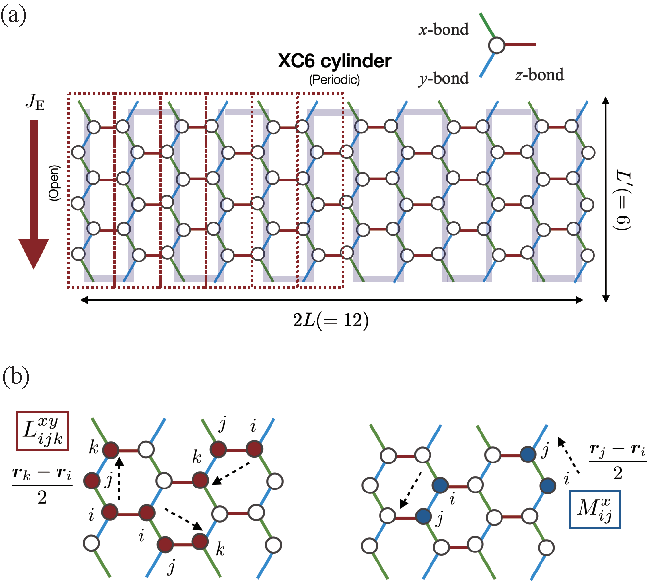
\includegraphics[width=\linewidth]{lattice.pdf}
  \end{center}
  \caption{(a) Schematic view of a XC6 honeycomb lattice consisting of 72 sites (XC6, $L=6$ lattice). Along the vertical direction, we impose the periodic bounray condition, while the left and the right boundraries are open. We consinder the thermalcurrent $J_{\mathrm{E}}$ in a downward direction indicated by the arrow. In the tensor network simulation, we consider a snake like matrix product operators indicated by the gray thick line behind the lattice. (b) Graphical representations of the three-body ($L$) and the two-body ($M$) terms in the definition of the thermal current \eqref{eq:def_J}.}
  \label{fig:lattice}
\end{figure}

\section{Method}
  \subsection{Thermal Hall conductivity}
  \begin{align}
   J_{\mathrm{E}} &=  i \left[\mathcal{H}, \bm{P}_{\mathrm{E}}\right] \notag \\
&= \sum_{\gamma,\gamma'}\sum_{\langle i,j,k\rangle_{\gamma,\gamma'}} \frac{\bm{r}_k-\bm{r}_i}{2}L_{ijk}^{\gamma\gamma'} + \sum_{\gamma}\sum_{\langle i,j\rangle_{\gamma}} \frac{\bm{r}_j-\bm{r}_i}{2}M_{ij}^{\gamma} 
   \label{eq:def_J}
  \end{align}
  \subsection{Tensor network method}
\begin{figure}
  \begin{center}
    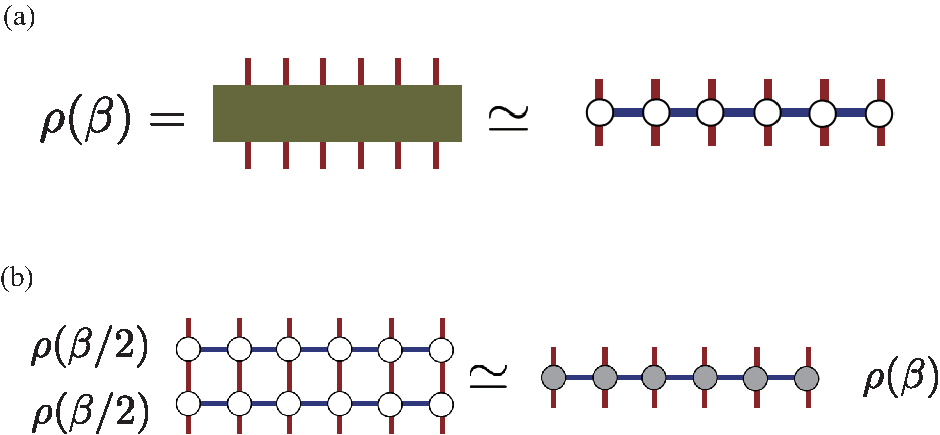
\includegraphics[width=\linewidth]{XTRG_MPO.pdf}
  \end{center}
  \caption{Tensor network diagram for the density operator approximation. (a) The density matrix is approximated as a matrix product operator with bond dimension $D$. Here, the horizontal line corresponds to the gray line in Fig.~\ref{fig:lattice}(a). (b) The density matrix at $\beta$ is calculated as $\rho(\beta)=\rho(\beta/2)\rho(\beta/2)$. The bond dimension of the obtained $\rho(\beta)$ is trunctaed to $D$ through the standard optimization procedure of MPS.}
  \label{fig:XTRG}
\end{figure}
  \subsection{Thermal pure quantum state}
In this section, we explain the basics of the canonical thermal quantum pure (cTPQ) state method.
We construct the 
cTPQ state $|\Phi_{\rm cTPQ}\rangle$ as follows:
\begin{align}
|\Phi_{\rm cTPQ}^{p}(\beta)\rangle = \exp\Big[-\frac{\beta}{2}H\Big]|\Phi_{\rm rand}^{p}\rangle,
\end{align}
where $\beta$ is inverse temperature and 
$|\Phi_{\rm rand}\rangle$ is the $p$th initial random vector, which uniformly distributed
on the $N_{\rm H}$ dimensional super sphere ($N_{\rm H}$ is the Hilbert dimension of 
the given systems).
Any local physical quantities at inverse temperature $\beta$
can be calculated as the expectation values of $|\Phi_{\rm cTPQ}(\beta)\rangle$, i.e.,
\begin{align}
\langle A(\beta)\rangle
=\frac{\langle \Phi_{\rm cTPQ}^{p}(\beta)|A|\Phi_{\rm cTPQ}^{p}(\beta)\rangle}
{\langle \Phi_{\rm cTPQ}^{p}(\beta)|\Phi_{\rm cTPQ}^{p}(\beta)\rangle}.
\end{align}
In the actual calculations, we calculate the 
cTPQ state as follows:
\begin{align}
&\exp\Big[-\frac{\beta}{2}H\Big]|\Phi_{\rm rand}^{p}\rangle=U(\Delta\tau)^{k}|\Phi_{\rm rand}^{p}\rangle,\\
&U(\Delta\tau)=\exp\Big[-\frac{\Delta\tau}{2}H\Big]\sim\sum_{n=0}^{n_{\rm max}}\frac{1}{n!}(-\frac{\Delta\tau}{2}H)^{n},\\
&\beta=k\Delta\tau,
\end{align}
where we take $n_{\rm max}=6$ and $\Delta\tau =0.02$.
We confirm that $n_{\rm max}$ ($\Delta\tau$) is sufficiently
large (small) for obtaining converged physical quantities 
in the calculated temperature region.

The cTPQ method gives the numerically exact
results within the statistical fluctuations,
which is defined by the statistical distribution of the initial random vectors.
To evaluate the fluctuations, i.e., the errors of the cTPQ method, 
we employ the bootstrap method.
Using the bootstrap method,
we evaluate the average values and 
error bars of physical quantities as follows.
\begin{enumerate}
\item Preparing $N_{\rm tot}$ random initial states and generating the cTPQ states.
\item Randomly choosing $P$ samples among $N_{\rm tot}$ cTPQ states allowing duplications. 
Repeating this procedure $M$ times and the mean value of the physical quantities $A$ 
at $m$th times is given by 
\begin{align}
A_{m}(\beta) = \frac{\sum_{p=1}^{P}\langle \Phi_{\rm cTPQ}^{p}(\beta)|A|\Phi_{\rm cTPQ}^{p}(\beta)\rangle}{\sum_{p=1}^{P}\langle \Phi_{\rm cTPQ}^{p}(\beta)|\Phi_{\rm cTPQ}^{p}(\beta)\rangle},
\end{align}
where $\langle A(\beta)\rangle_{p}$ is the physical quantities calculated by the cTPQ state 
which is generated by $p$th initial states.
\item From $A_{m}(\beta)$, the 
average value $\bar{A}(\beta)$
and the standard deviations (error bars, $\sigma[A(\beta)]$ ) are 
evaluated as
\begin{align}
&\bar{A}(\beta) = \frac{1}{M}\sum_{m=1}^{M}A_{m}(\beta), \\
&\sigma[A(\beta)] = \Big[\frac{1}{M-1}(\sum_{m=1}^{M}A_{m}(\beta)^2-\bar{A}(\beta)^2)\Big]^{1/2}.
\end{align}
\end{enumerate}
  \subsection{Classical Monte Carlo simulation}


\section{Result}
  \subsection{Pure Kitaev model}
   \subsubsection{Ferromagnetic case}
\begin{figure*}
  \begin{center}
    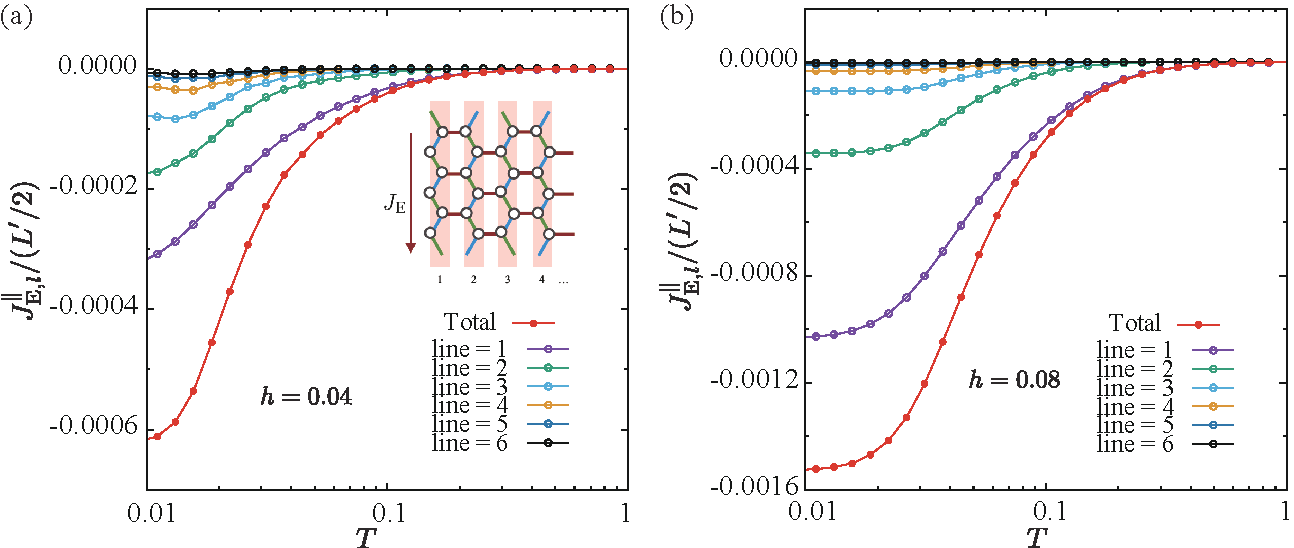
\includegraphics[width=0.9\linewidth]{J_line_all.pdf}
  \end{center}
  \caption{Temperature dependence of the energy current of the ferromagnetic Kitaev model under (a) $h=0.04$ and (b) $h=0.08$. In adittion to the total energy current, contribution from each line is presented.}
  \label{fig:J_line}
\end{figure*}

\begin{figure}
  \begin{center}
    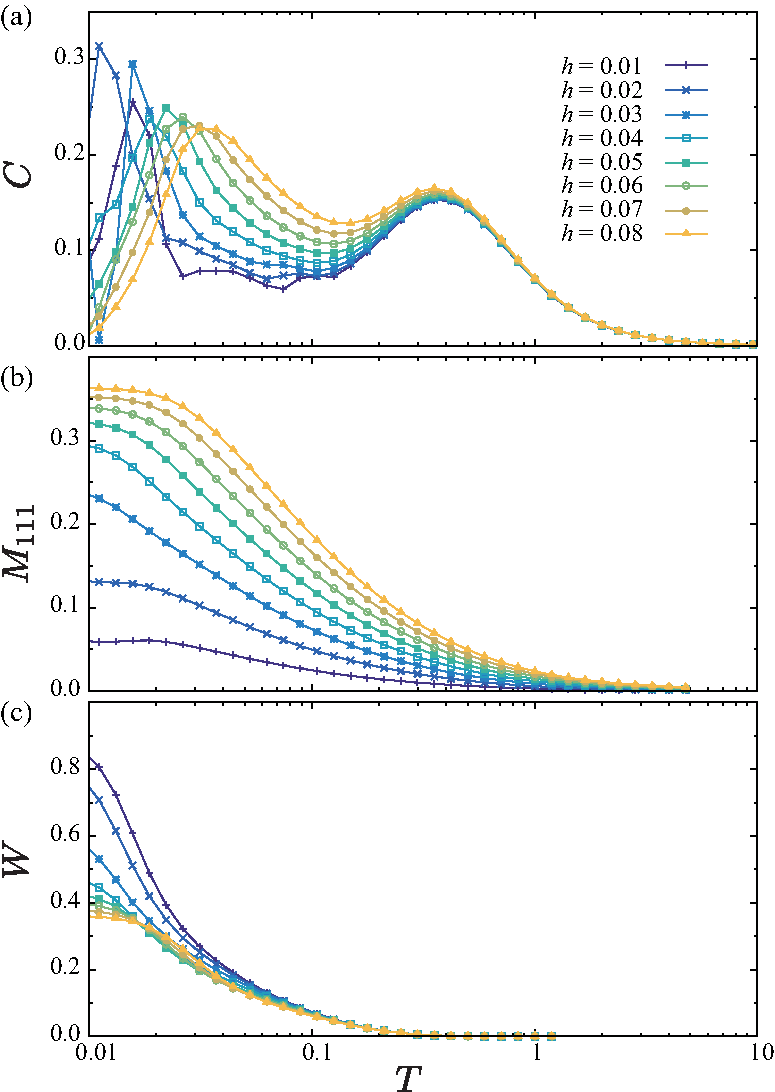
\includegraphics[width=0.9\linewidth]{plot_CMF.pdf}
  \end{center}
  \caption{Temperature dependence of (a) the specific heat (b) the magnetic moment, and (c) the flux of the ferromagnetic Kitaev model for various external magnetic field parallel to $[111]$ direction.}
  \label{fig:CMF_pure}
\end{figure}
\begin{figure}
  \begin{center}
    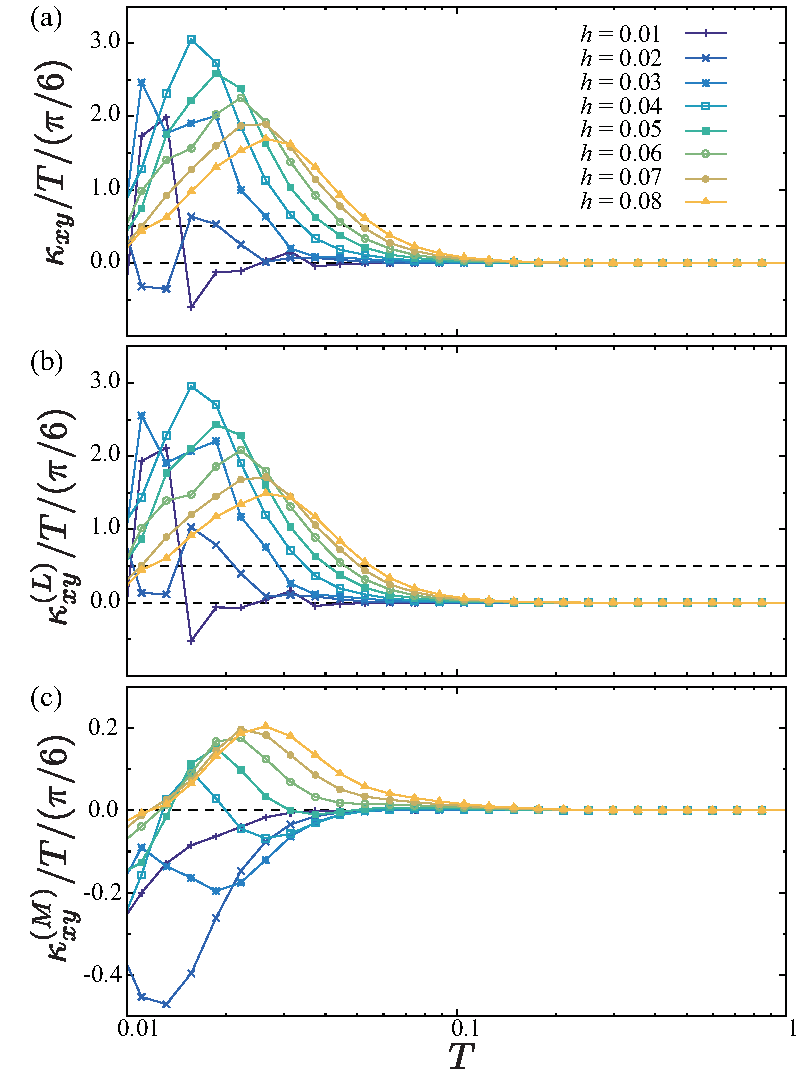
\includegraphics[width=0.9\linewidth]{plot_k_all.pdf}
  \end{center}
  \caption{(a) Temperature dependence of $\kappa_{xy}/T$ of the ferromagnetic Kitaev model for various magnetic fields parallel to $[111]$ direction. Two horizontal dashed lines indicate $\kappa_{xy}/T = 0$ and the half-quantized value. (b,c) Contributions from the three-body ($L$) and and the two-body ($M$) terms, respectively.}
  \label{fig:k_all_pure}
\end{figure}


   \subsubsection{Field angle dependence}
\begin{figure}
  \begin{center}
    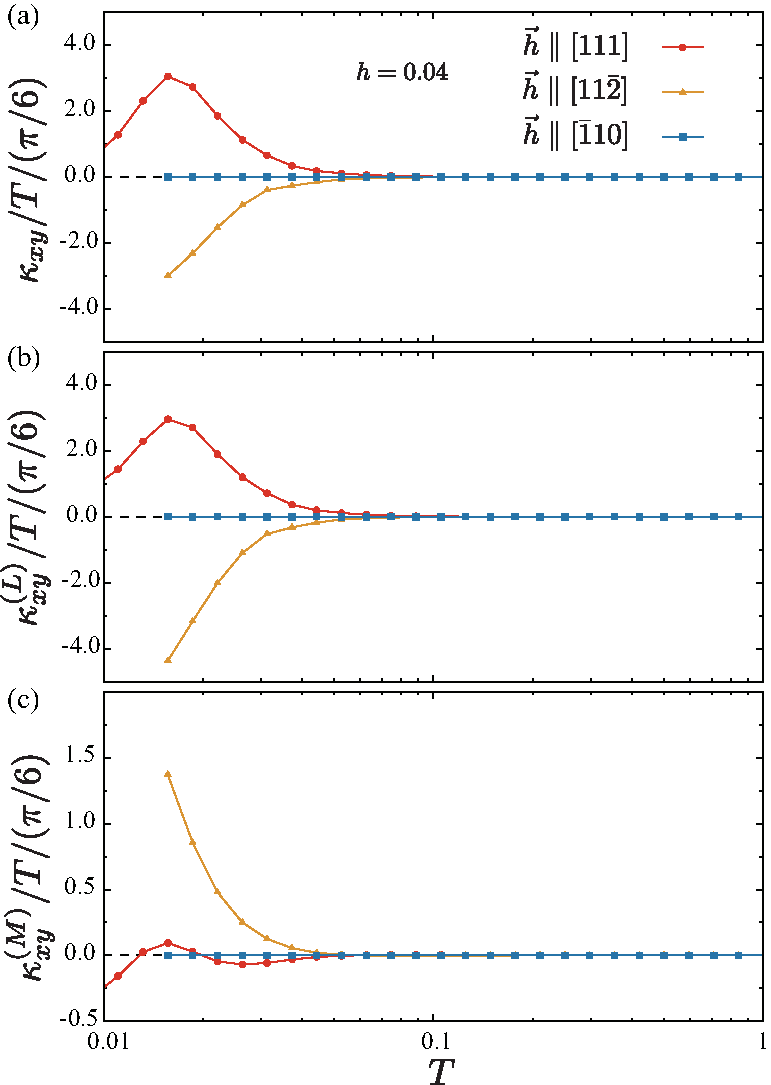
\includegraphics[width=0.9\linewidth]{plot_k_all_h0.04_ab.pdf}
  \end{center}
  \caption{(top) Temperature dependence of $\kappa_{xy}/T$ of the ferromagnetic Kitaev model under magnetic fields parallel to $[111]$, $[11\bar{2}]$, and $[1\bar{1}0]$ with $|h|=0.04$. The horizontal dashed line indicates $\kappa_{xy}/T = 0$. The middle and the bottom figures are contributions from the three-body ($L$) and and the two-body ($M$) terms, respectively.}
  \label{fig:k_all_h0.04_ab}
\end{figure}

\begin{figure}
  \begin{center}
    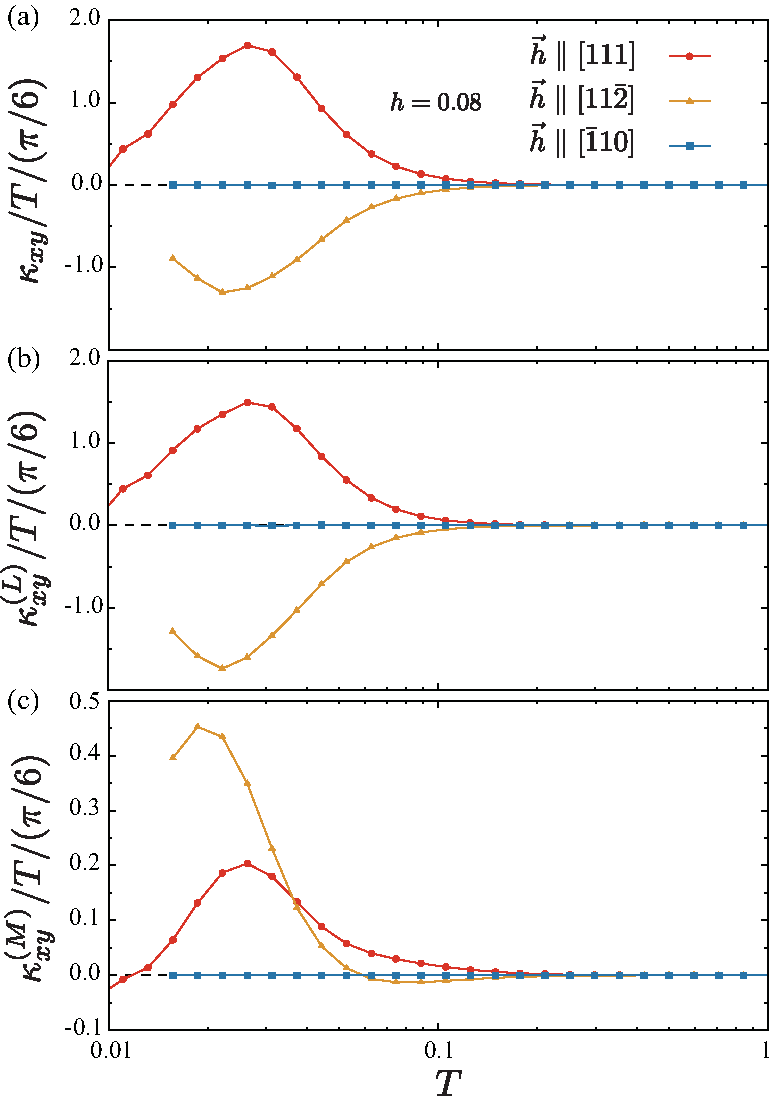
\includegraphics[width=0.9\linewidth]{plot_k_all_h0.08_ab.pdf}
  \end{center}
  \caption{(top) Temperature dependence of $\kappa_{xy}/T$ of the ferromagnetic Kitaev model under magnetic fields parallel to $[111]$, $[11\bar{2}]$, and $[1\bar{1}0]$ with $|h|=0.08$. The horizontal dashed line indicates $\kappa_{xy}/T = 0$. The middle and the bottom figures are contributions from the three-body ($L$) and and the two-body ($M$) terms, respectively.}
  \label{fig:k_all_h0.08_ab}
\end{figure}
  \subsection{Effect of non-Kitaev interactions}
   \subsubsection{Symmetric off-dinagonal interaction $\Gamma$} 
\begin{figure}
  \begin{center}
    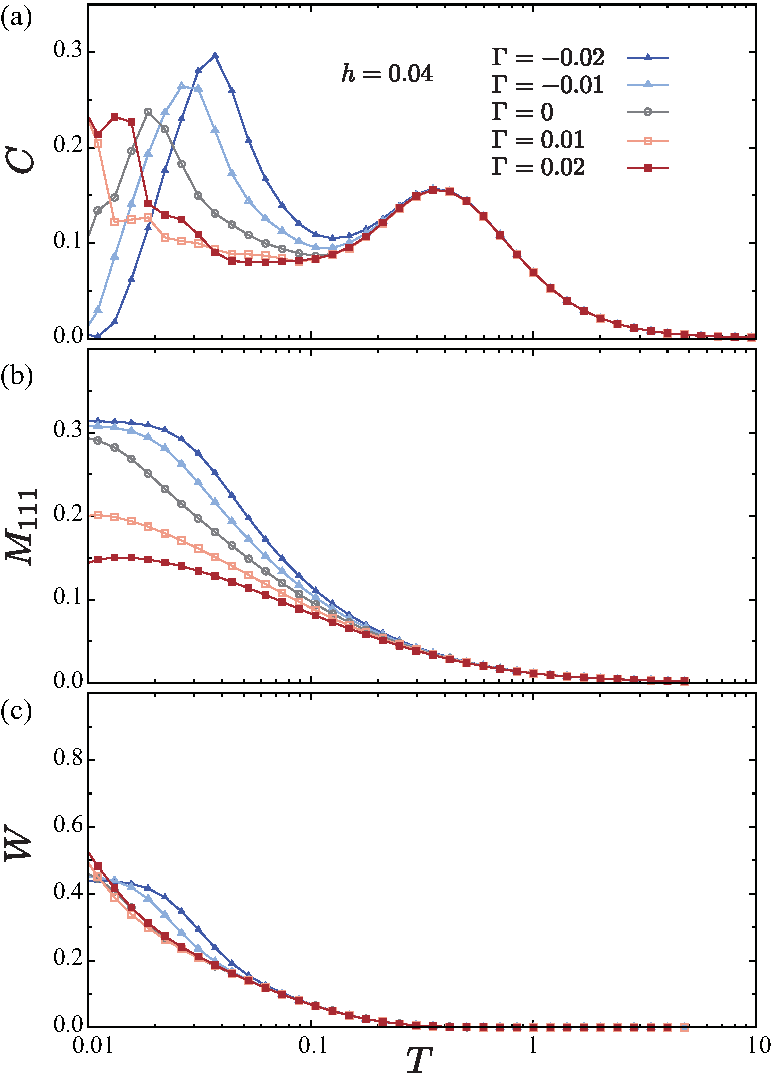
\includegraphics[width=0.9\linewidth]{plot_CMF_h0.04_G.pdf}
  \end{center}
  \caption{Temperature dependence of (a) the specific heat (b) the magnetic moment, and (c) the flux of the ferromagnetic Kitaev model with a weak $\Gamma$ under a magnetic field parallel to $[111]$ direction. The amplitude of the magnetic field is $|h|=0.04$.}
  \label{fig:CMF_h0.04_G}
\end{figure}
\begin{figure}
  \begin{center}
    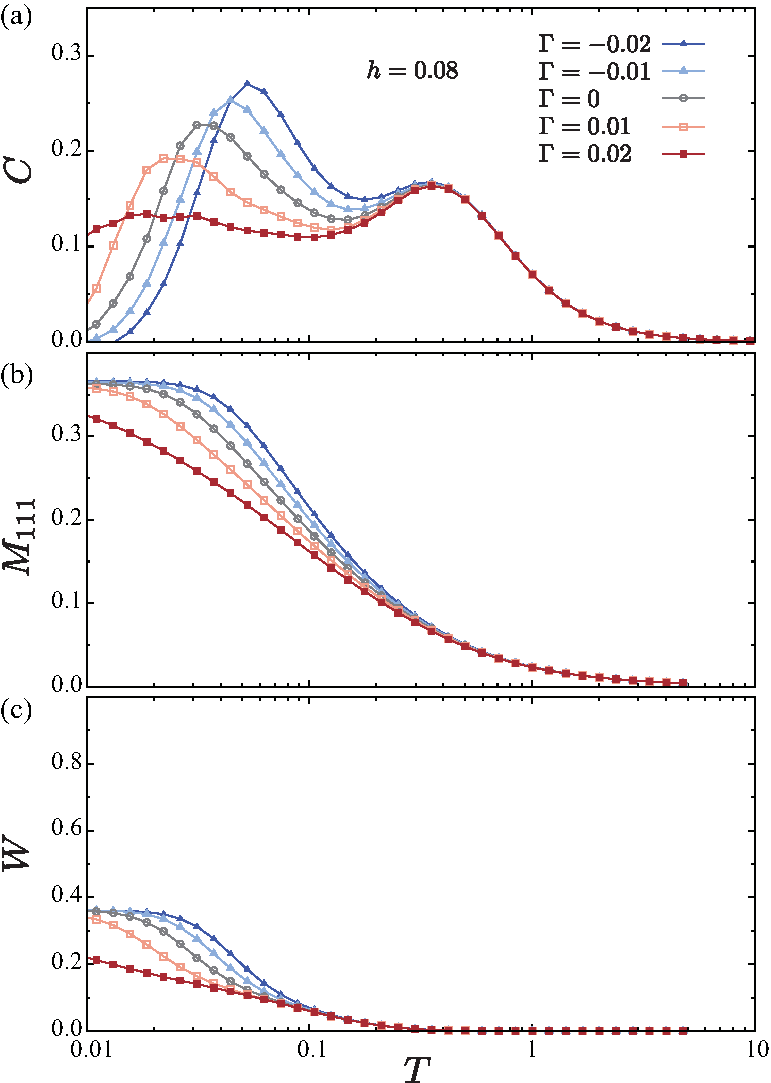
\includegraphics[width=0.9\linewidth]{plot_CMF_h0.08_G.pdf}
  \end{center}
  \caption{Temperature dependence of (a) the specific heat (b) the magnetic moment, and (c) the flux of the ferromagnetic Kitaev model with a weak $\Gamma$ under a magnetic field parallel to $[111]$ direction. The amplitude of the magnetic field is $|h|=0.08$.}
  \label{fig:CMF_h0.08_G}
\end{figure}

\begin{figure}
  \begin{center}
    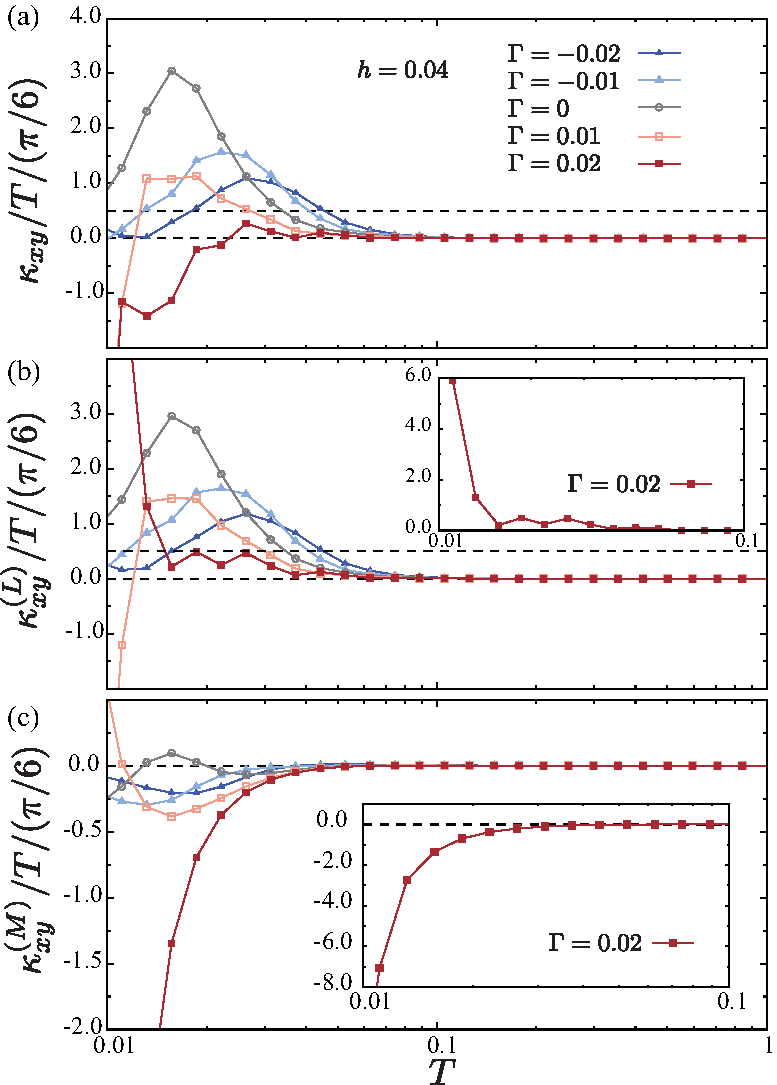
\includegraphics[width=0.9\linewidth]{plot_k_all_h0.04_G.pdf}
  \end{center}
  \caption{(a) Temperature dependence of $\kappa_{xy}/T$ of the ferromagnetic Kitaev model with as weak $\Gamma$ interaction under a magnetic field parallel to $[111]$. The amplitude of the magnetic field is set to $|h|=0.04$. Two horizontal dashed lines indicate $\kappa_{xy}/T = 0$ and the half-quantized value. (b, c) Contributions from the three-body ($L$) and and the two-body ($M$) terms, respectively.The insets show magnified views for $\Gamma = 0.02$.}
  \label{fig:k_all_h0.04_G}
\end{figure}
\begin{figure}
  \begin{center}
    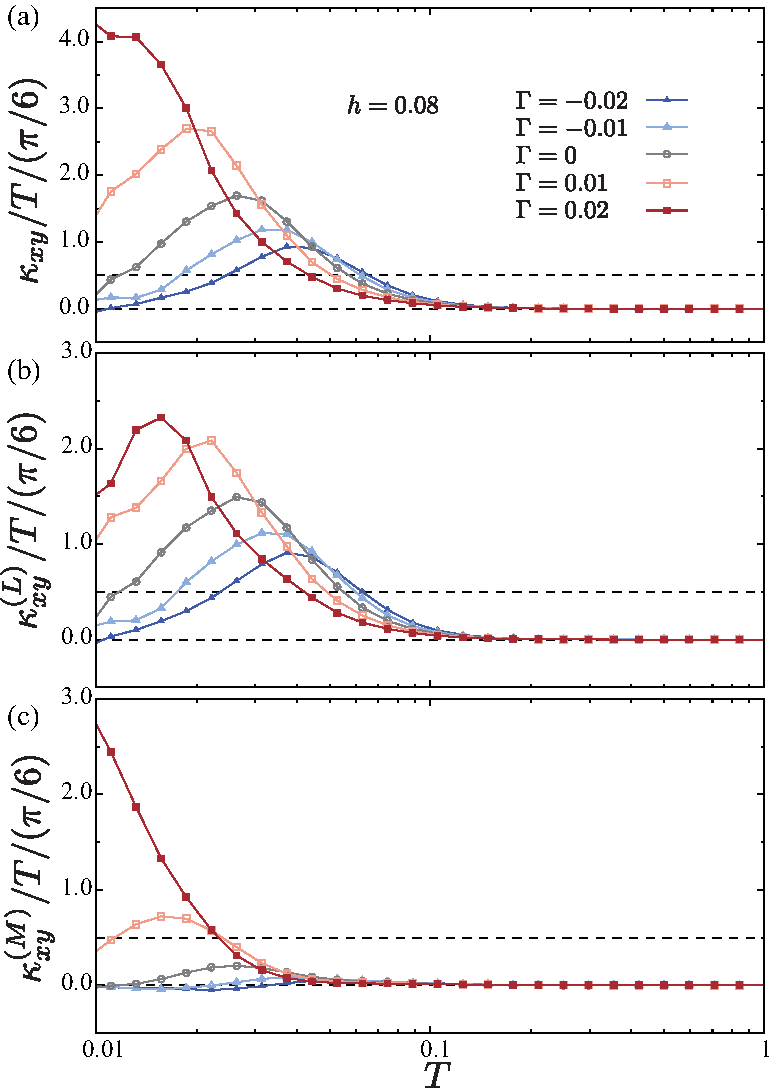
\includegraphics[width=0.9\linewidth]{plot_k_all_h0.08_G.pdf}
  \end{center}
  \caption{(a) Temperature dependence of $\kappa_{xy}/T$ of the ferromagnetic Kitaev model with as weak $\Gamma$ interaction under a magnetic field parallel to $[111]$. The amplitude of the magnetic field is set to $|h|=0.08$. Two horizontal dashed lines indicate $\kappa_{xy}/T = 0$ and the half-quantized value. (b, c) Contributions from the three-body ($L$) and and the two-body ($M$) terms, respectively.}
  \label{fig:k_all_h0.08_G}
\end{figure}
   
   

   \subsubsection{Symmetric off-dinagonal interaction $\Gamma'$}
\begin{figure}
  \begin{center}
    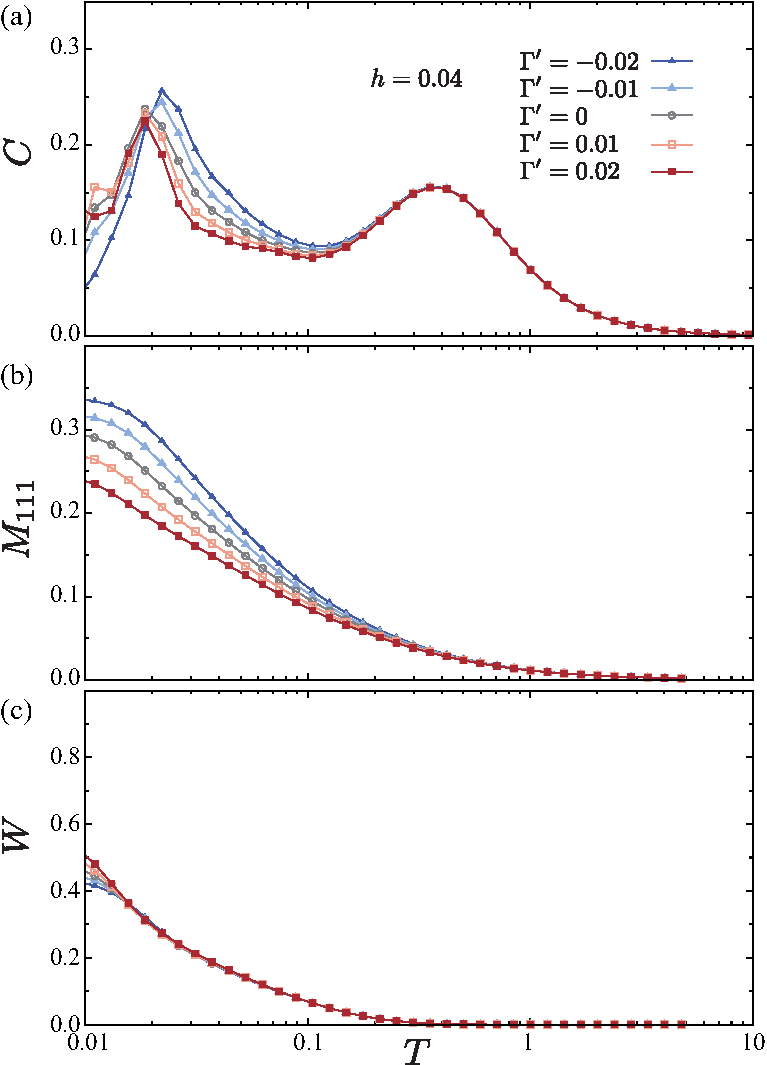
\includegraphics[width=0.9\linewidth]{plot_CMF_h0.04_Gp.pdf}
  \end{center}
  \caption{Temperature dependence of (a) the specific heat (b) the magnetic moment, and (c) the flux of the ferromagnetic Kitaev model with a weak $\Gamma'$ under a magnetic field parallel to $[111]$ direction. The amplitude of the magnetic field is $|h|=0.04$.}
  \label{fig:CMF_h0.04_Gp}
\end{figure}
\begin{figure}
  \begin{center}
    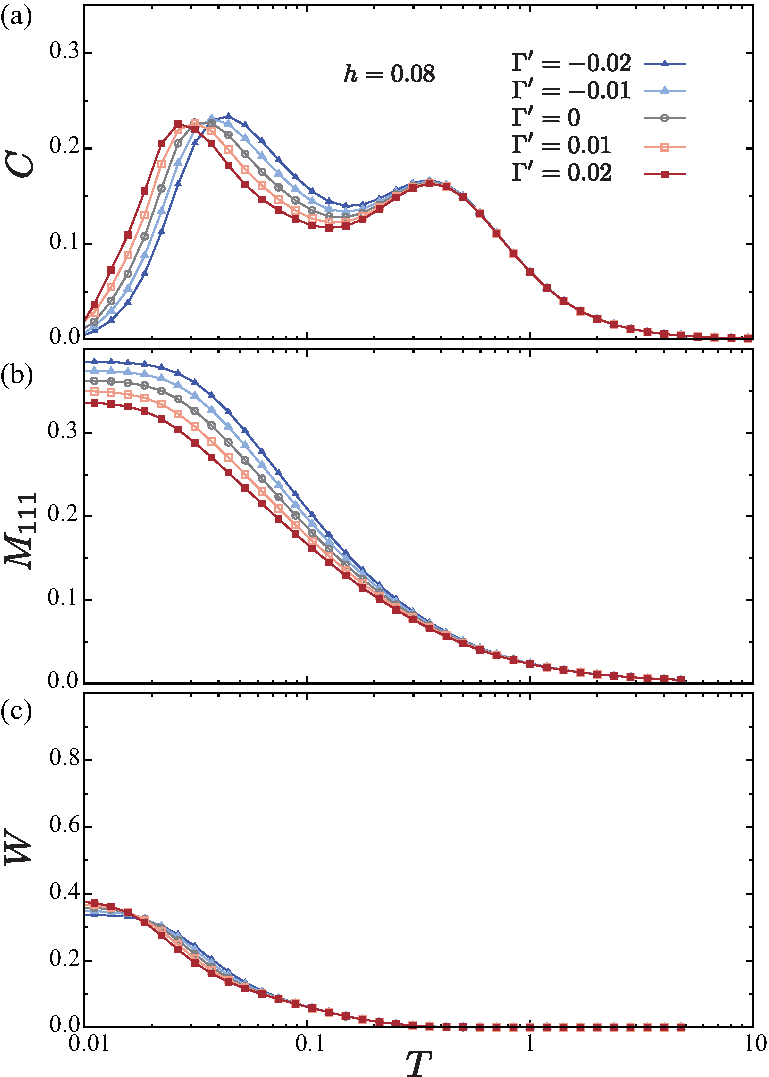
\includegraphics[width=0.9\linewidth]{plot_CMF_h0.08_Gp.pdf}
  \end{center}
  \caption{Temperature dependence of (a) the specific heat (b) the magnetic moment, and (c) the flux of the ferromagnetic Kitaev model with a weak $\Gamma'$ under a magnetic field parallel to $[111]$ direction. The amplitude of the magnetic field is $|h|=0.08$.}
  \label{fig:CMF_h0.08_Gp}
\end{figure}

\begin{figure}
  \begin{center}
    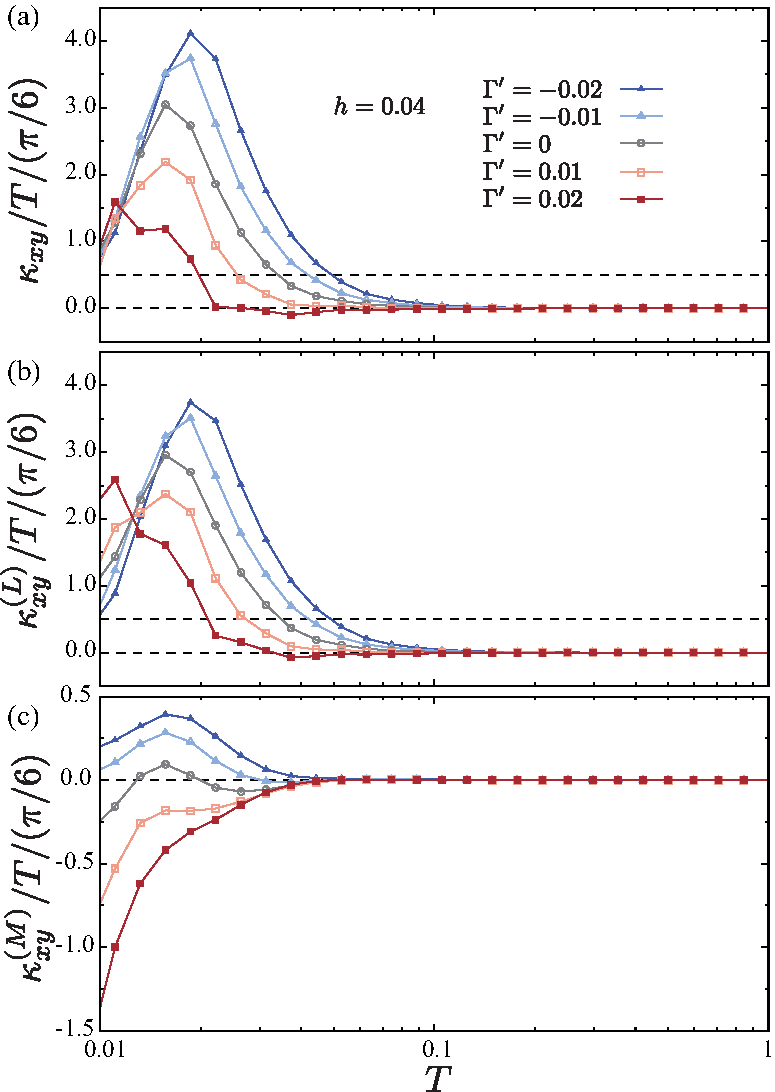
\includegraphics[width=0.9\linewidth]{plot_k_all_h0.04_Gp.pdf}
  \end{center}
  \caption{(a) Temperature dependence of $\kappa_{xy}/T$ of the ferromagnetic Kitaev model with as weak $\Gamma'$ interaction under a magnetic field parallel to $[111]$. The amplitude of the magnetic field is set to $|h|=0.04$. Two horizontal dashed lines indicate $\kappa_{xy}/T = 0$ and the half-quantized value. (b, c) Contributions from the three-body ($L$) and and the two-body ($M$) terms, respectively.}
  \label{fig:k_all_h0.04_Gp}
\end{figure}
\begin{figure}
  \begin{center}
    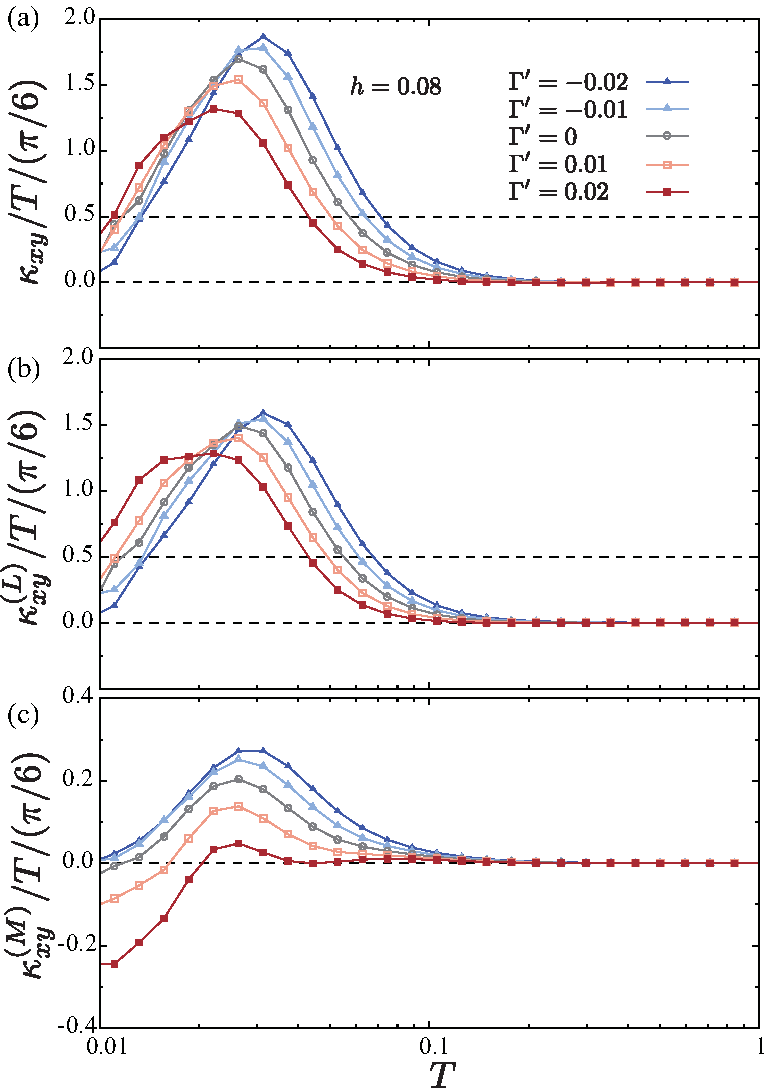
\includegraphics[width=0.9\linewidth]{plot_k_all_h0.08_Gp.pdf}
  \end{center}
  \caption{(a) Temperature dependence of $\kappa_{xy}/T$ of the ferromagnetic Kitaev model with as weak $\Gamma'$ interaction under a magnetic field parallel to $[111]$. The amplitude of the magnetic field is set to $|h|=0.08$. Two horizontal dashed lines indicate $\kappa_{xy}/T = 0$ and the half-quantized value. (b, c) Contributions from the three-body ($L$) and and the two-body ($M$) terms, respectively.}
  \label{fig:k_all_h0.08_Gp}
\end{figure}
  \subsection{Classical limit}

\begin{figure}[tbh] 
\begin{center} 
\includegraphics[width=0.9\linewidth]{fig_K-1.0_G0.00_Gp0.00_c.pdf}
\vspace{-0.5cm} 
\caption{Temperature dependence of (a) the specific heat, (b) the total magnetization, and
(c) the thermal Hall conductivity $\kappa_{xy}$ for several magnetic fields along the $[111]$ direction in the classical Kitaev model.
(d),(e) Temperature dependence of the two components, $(L)$ and $(M)$, of the thermal Hall conductivity.}
\label{fig_classical_hdep}
\end{center}
\end{figure}


\begin{figure}[tbh] 
\begin{center} 
\includegraphics[width=0.9\linewidth]{fig_K-1.0_G0.00_Gp0.00_h0.04.pdf}
\vspace{-0.5cm} 
\caption{Temperature dependence of (a) the specific heat, (b) the total magnetization, and
(c) the thermal Hall conductivity $\kappa_{xy}$ in the classical Kitaev model under the magnetic field parallel to $[111]$, $[11\bar{2}]$, and $[\bar{1}10]$ with $h=0.04$.
(d),(e) Temperature dependence of the two components, $(L)$ and $(M)$, of the thermal Hall conductivity.}
\label{fig_classical_adep004}
\end{center}
\end{figure}


\begin{figure}[tbh] 
\begin{center} 
\includegraphics[width=0.9\linewidth]{fig_K-1.0_G0.00_Gp0.00_h0.08.pdf}
\vspace{-0.5cm} 
\caption{Temperature dependence of (a) the specific heat, (b) the total magnetization, and
(c) the thermal Hall conductivity $\kappa_{xy}$ in the classical Kitaev model under the magnetic field parallel to $[111]$, $[11\bar{2}]$, and $[\bar{1}10]$ with $h=0.08$.
(d),(e) Temperature dependence of the two components, $(L)$ and $(M)$, of the thermal Hall conductivity.}
\label{fig_classical_adep008}
\end{center}
\end{figure}



\begin{figure}[tbh] 
\begin{center} 
\includegraphics[width=0.9\linewidth]{fig_K-1.0_Gp0.00_h0.04.pdf}
\vspace{-0.5cm} 
\caption{Temperature dependence of (a) the specific heat, (b) the total magnetization, and
(c) the thermal Hall conductivity $\kappa_{xy}$ in the classical Kitaev-$\Gamma$ model under the magnetic field with $h=0.04$.
(d),(e) Temperature dependence of the two components, $(L)$ and $(M)$, of the thermal Hall conductivity.}
\label{fig_classical_gdep004}
\end{center}
\end{figure}


\begin{figure}[tbh] 
\begin{center} 
\includegraphics[width=0.9\linewidth]{fig_K-1.0_Gp0.00_h0.08.pdf}
\vspace{-0.5cm} 
\caption{Temperature dependence of (a) the specific heat, (b) the total magnetization, and
(c) the thermal Hall conductivity $\kappa_{xy}$ in the classical Kitaev-$\Gamma$ model under the magnetic field with $h=0.08$.
(d),(e) Temperature dependence of the two components, $(L)$ and $(M)$, of the thermal Hall conductivity.}
\label{fig_classical_gdep008}
\end{center}
\end{figure}
  


\begin{figure}[tbh] 
\begin{center} 
\includegraphics[width=0.9\linewidth]{fig_K-1.0_G0.00_h0.04.pdf}
\vspace{-0.5cm} 
\caption{Temperature dependence of (a) the specific heat, (b) the total magnetization, and
(c) the thermal Hall conductivity $\kappa_{xy}$ in the classical Kitaev-$\Gamma'$ model under the magnetic field with $h=0.04$.
(d),(e) Temperature dependence of the two components, $(L)$ and $(M)$, of the thermal Hall conductivity.}
\label{fig_classical_gpdep004}
\end{center}
\end{figure}


\begin{figure}[tbh] 
\begin{center} 
\includegraphics[width=0.9\linewidth]{fig_K-1.0_G0.00_h0.08.pdf}
\vspace{-0.5cm} 
\caption{Temperature dependence of (a) the specific heat, (b) the total magnetization, and
(c) the thermal Hall conductivity $\kappa_{xy}$ in the classical Kitaev-$\Gamma'$ model under the magnetic field with $h=0.08$.
(d),(e) Temperature dependence of the two components, $(L)$ and $(M)$, of the thermal Hall conductivity.}
\label{fig_classical_gpdep008}
\end{center}
\end{figure}

  \subsection{Summary of temperature field dependence}
\begin{figure*}
  \begin{center}
    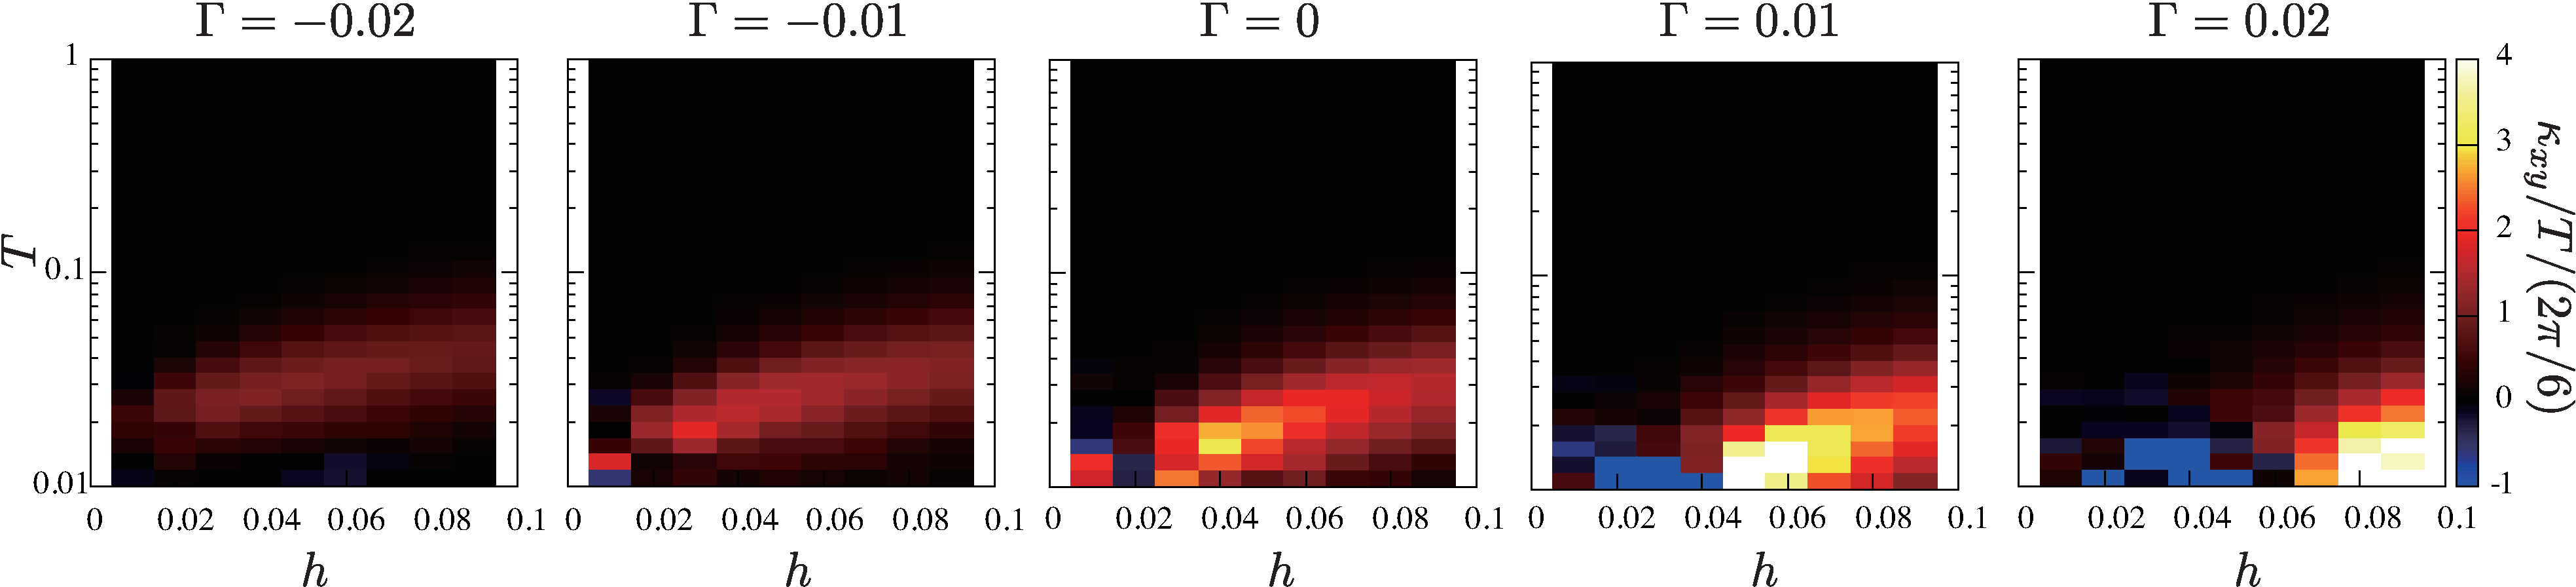
\includegraphics[width=\linewidth]{color_map_G.pdf}
  \end{center}
  \caption{Color maps of $\kappa_{xy}/T$ for ferromagnetic Kitaev model with $\Gamma = 0, \pm 0.01, \pm 0.02$ with various magnetic fields and temperatures.}
  \label{fig:color_map_G}
\end{figure*}

\begin{figure*}
  \begin{center}
    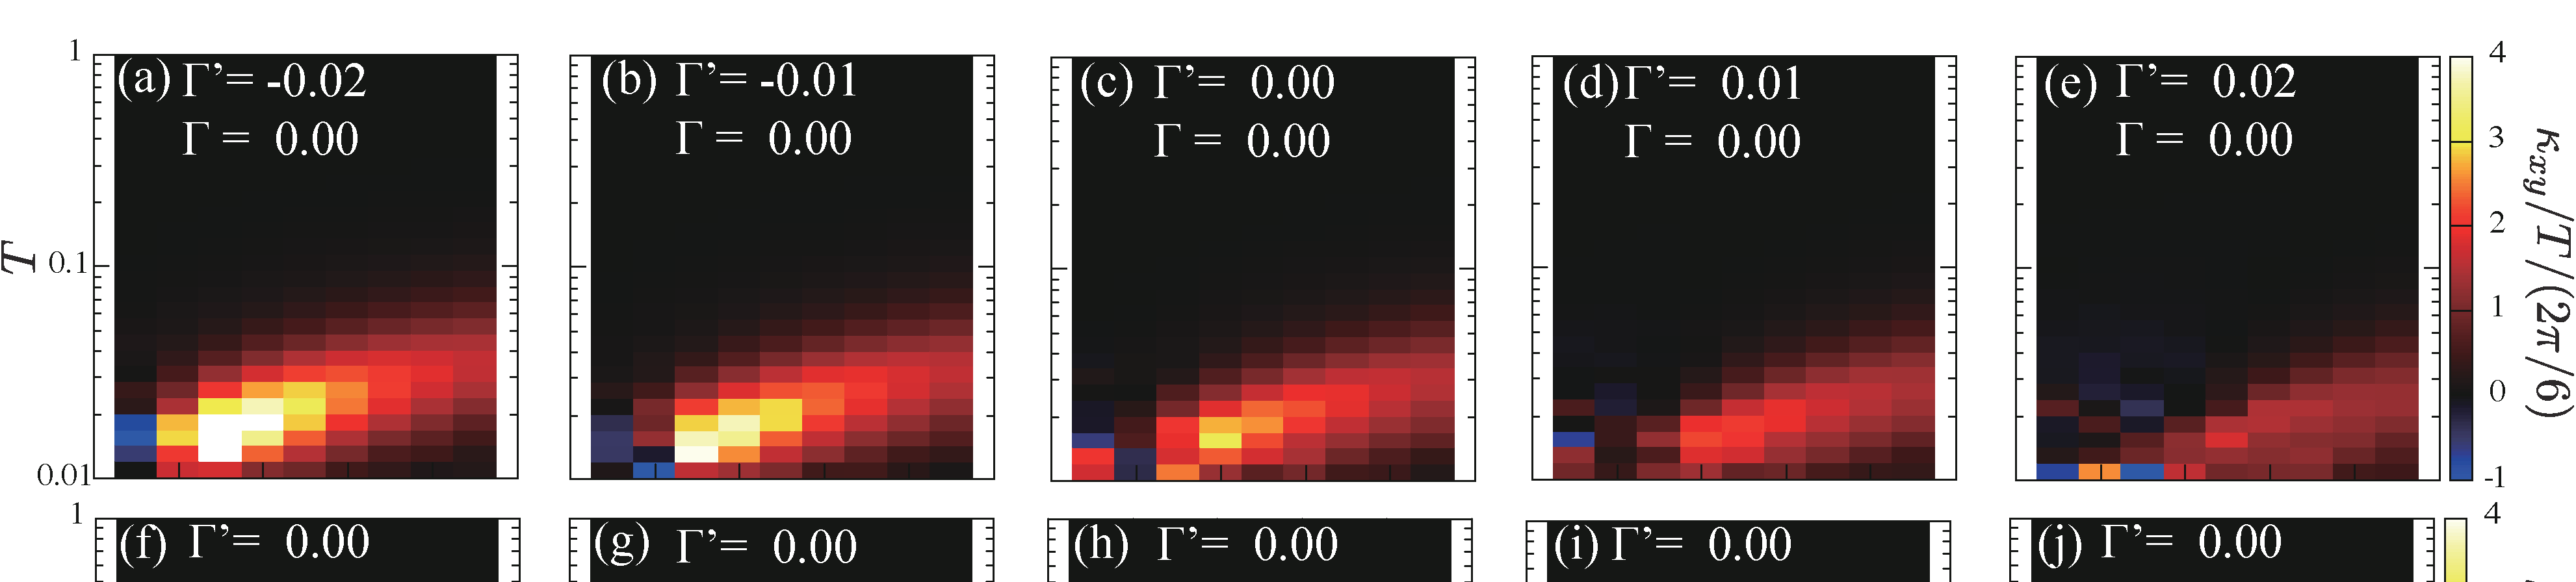
\includegraphics[width=\linewidth]{color_map_Gp.pdf}
  \end{center}
  \caption{Color maps of $\kappa_{xy}/T$ for ferromagnetic Kitaev model with $\Gamma' = 0, \pm 0.01, \pm 0.02$ with various magnetic fields and temperatures.}
  \label{fig:color_map_Gp}
\end{figure*}
 
  
\section{Summary}

\appendix

\section{Benchmark on tensor network method}


\begin{figure}
  \begin{center}
    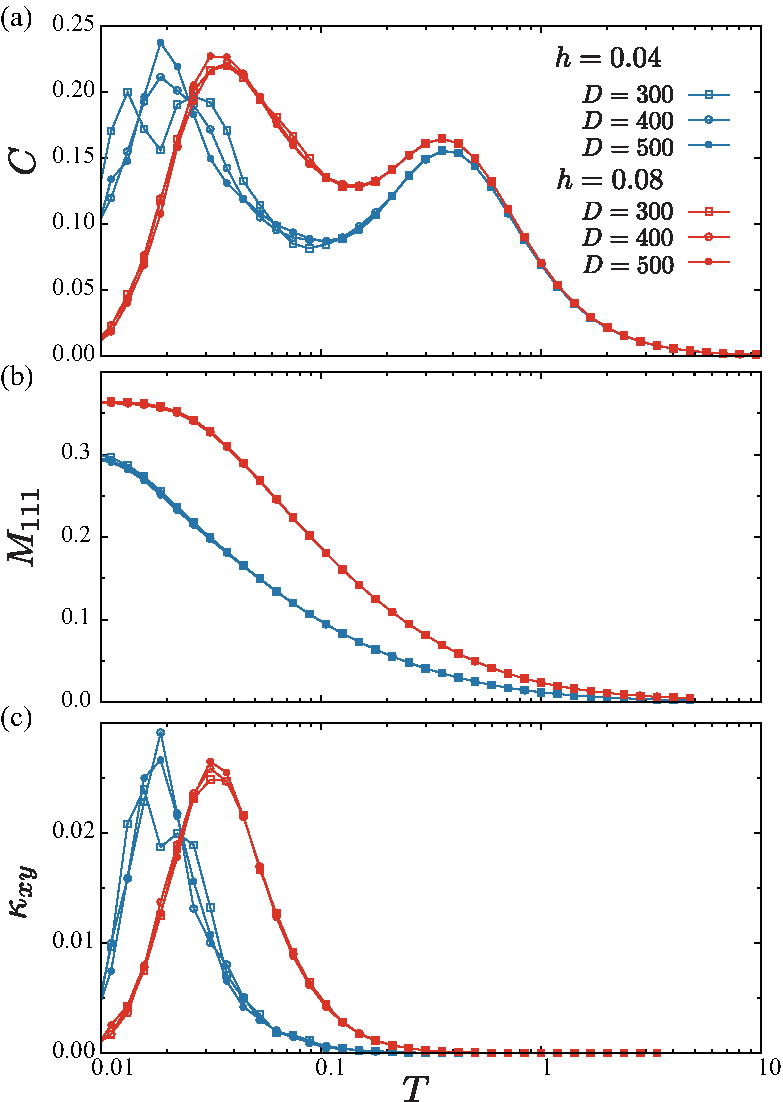
\includegraphics[width=0.9\linewidth]{plot_CMk.pdf}
  \end{center}
  \caption{Temperature dependence of (a) the specific heat (b) the magnetic moment, and (c) the thermal Hall conductivity of the ferromagnetic Kitaev model for the external magnetic field $h=0.04$ and $h=0.08$ parallel to $[111]$ direction with different bond-dimenisions $D=300, 400, 500$. The lattice is XC6, $L=6$}
  \label{fig:CMk_XC6}
\end{figure}
\begin{figure}
  \begin{center}
    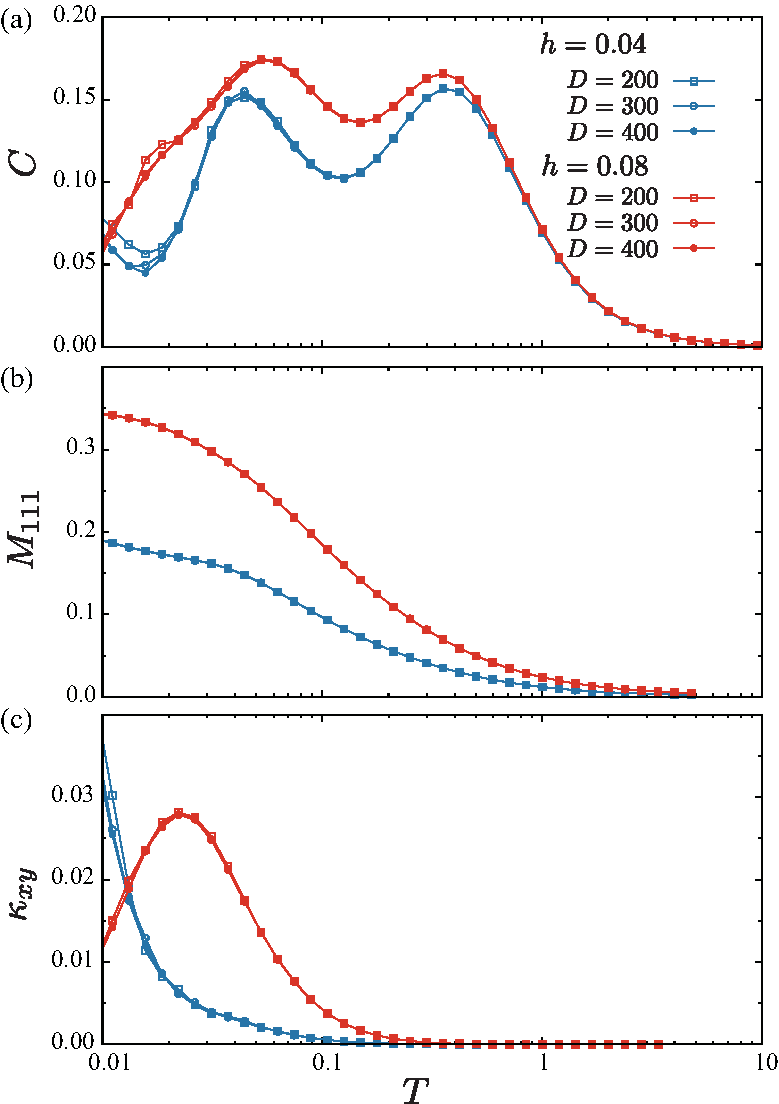
\includegraphics[width=0.9\linewidth]{plot_CMk_XC4.pdf}
  \end{center}
  \caption{Temperature dependence of (a) the specific heat (b) the magnetic moment, and (c) the thermal Hall conductivity of the ferromagnetic Kitaev model for the external magnetic field $h=0.04$ and $h=0.08$ parallel to $[111]$ direction with different bond-dimenisions $D=200, 300, 400$. The lattice is XC4, $L=8$}
  \label{fig:CMk_XC4}
\end{figure}


\begin{figure}
  \begin{center}
    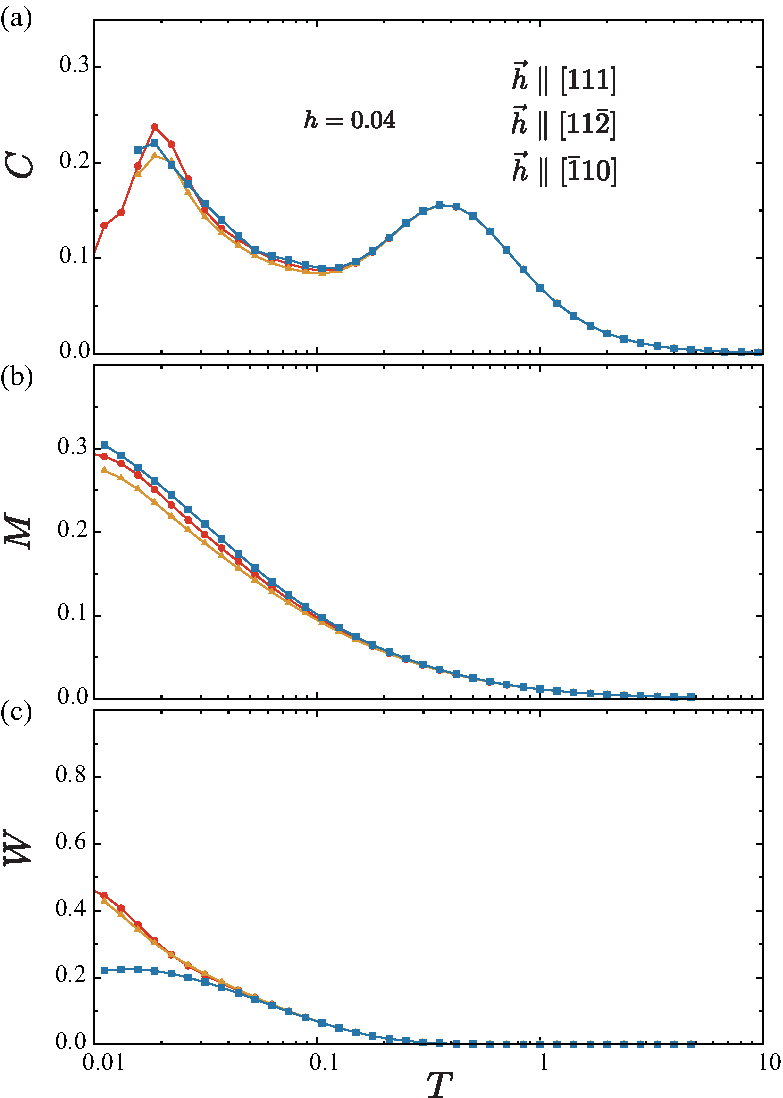
\includegraphics[width=0.9\linewidth]{plot_CMF_h0.04_ab.pdf}
  \end{center}
  \caption{Temperature dependence of (a) the specific heat (b) the magnetic moment, and (c) the flux of the ferromagnetic Kitaev model under magnetic fields parallel to $[111]$, $[11\bar{2}]$, and $[1\bar{1}0]$ with $|h|=0.04$.}
  \label{fig:CMF_h0.04_ab}
\end{figure}
\begin{figure}
  \begin{center}
    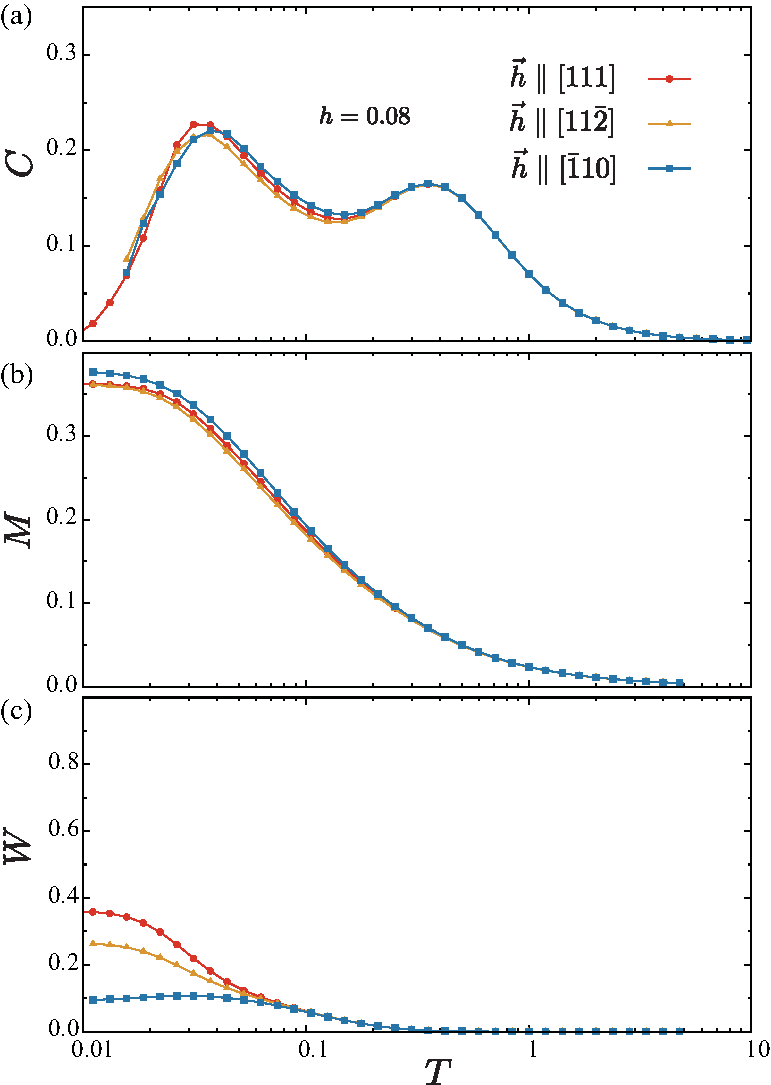
\includegraphics[width=0.9\linewidth]{plot_CMF_h0.08_ab.pdf}
  \end{center}
  \caption{Temperature dependence of (a) the specific heat (b) the magnetic moment, and (c) the flux of the ferromagnetic Kitaev model under magnetic fields parallel to $[111]$, $[11\bar{2}]$, and $[1\bar{1}0]$ with $|h|=0.08$.}
  \label{fig:CMF_h0.08_ab}
\end{figure}


\begin{figure*}
  \begin{center}
    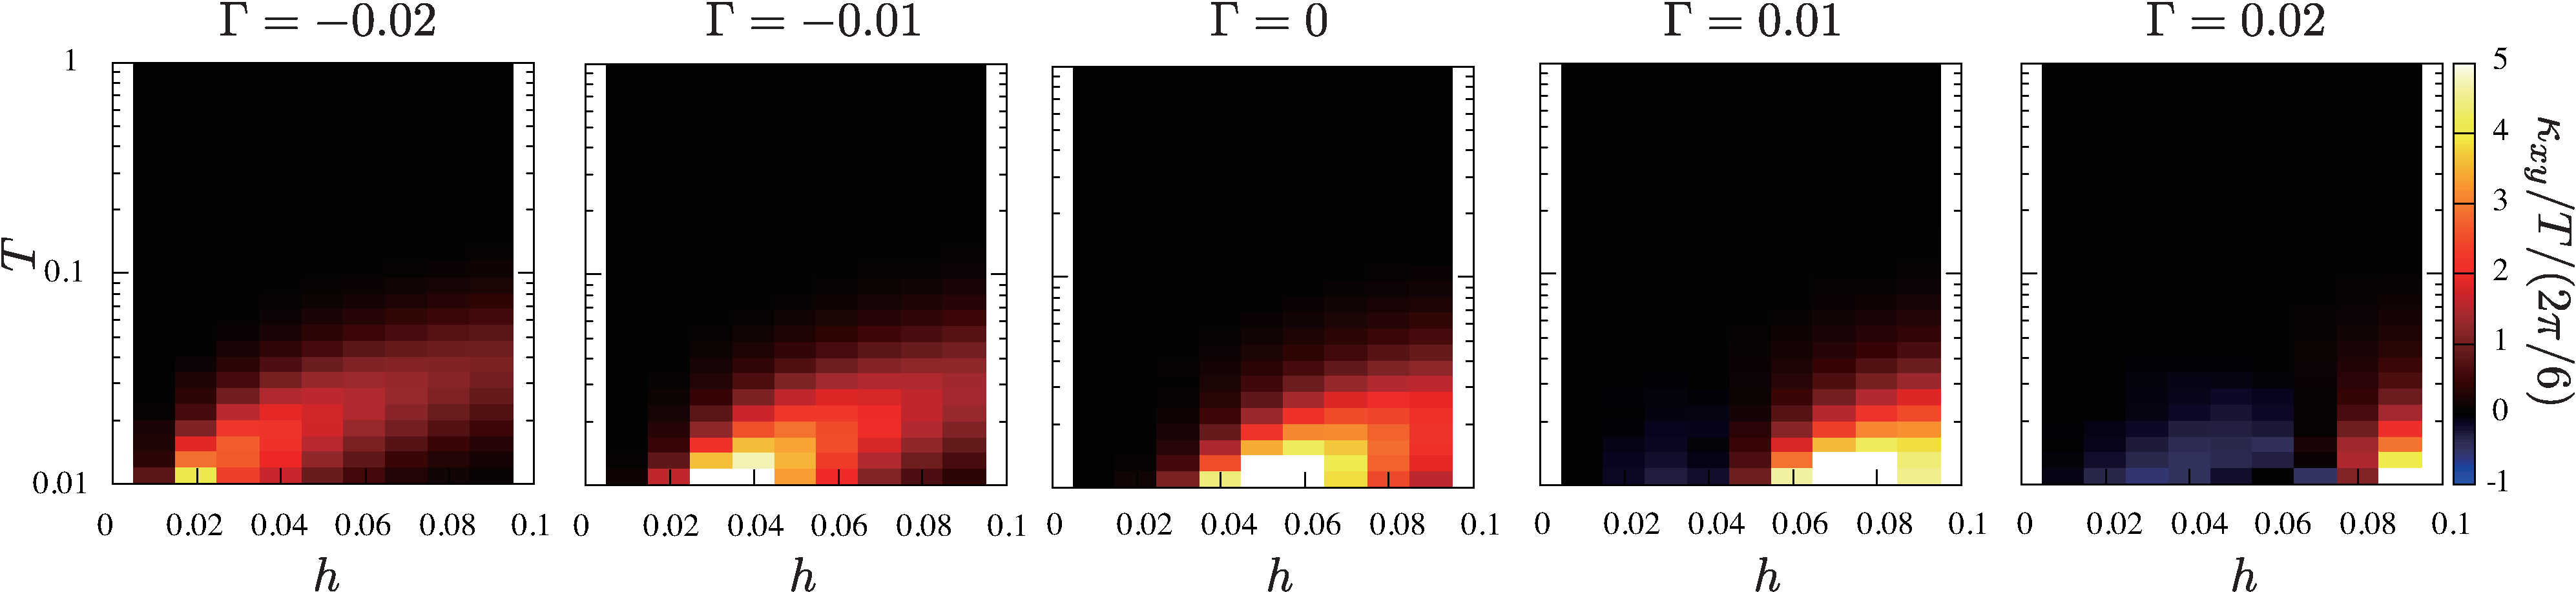
\includegraphics[width=\linewidth]{color_map_G_XC4.pdf}
  \end{center}
  \caption{Color maps of $\kappa_{xy}/T$ for ferromagnetic Kitaev model with $\Gamma = 0, \pm 0.01, \pm 0.02$ with various magnetic fields and temperatures. The lattice is XC4, $L=8$.}
  \label{fig:color_map_G_XC4}
\end{figure*}

\begin{figure*}
  \begin{center}
    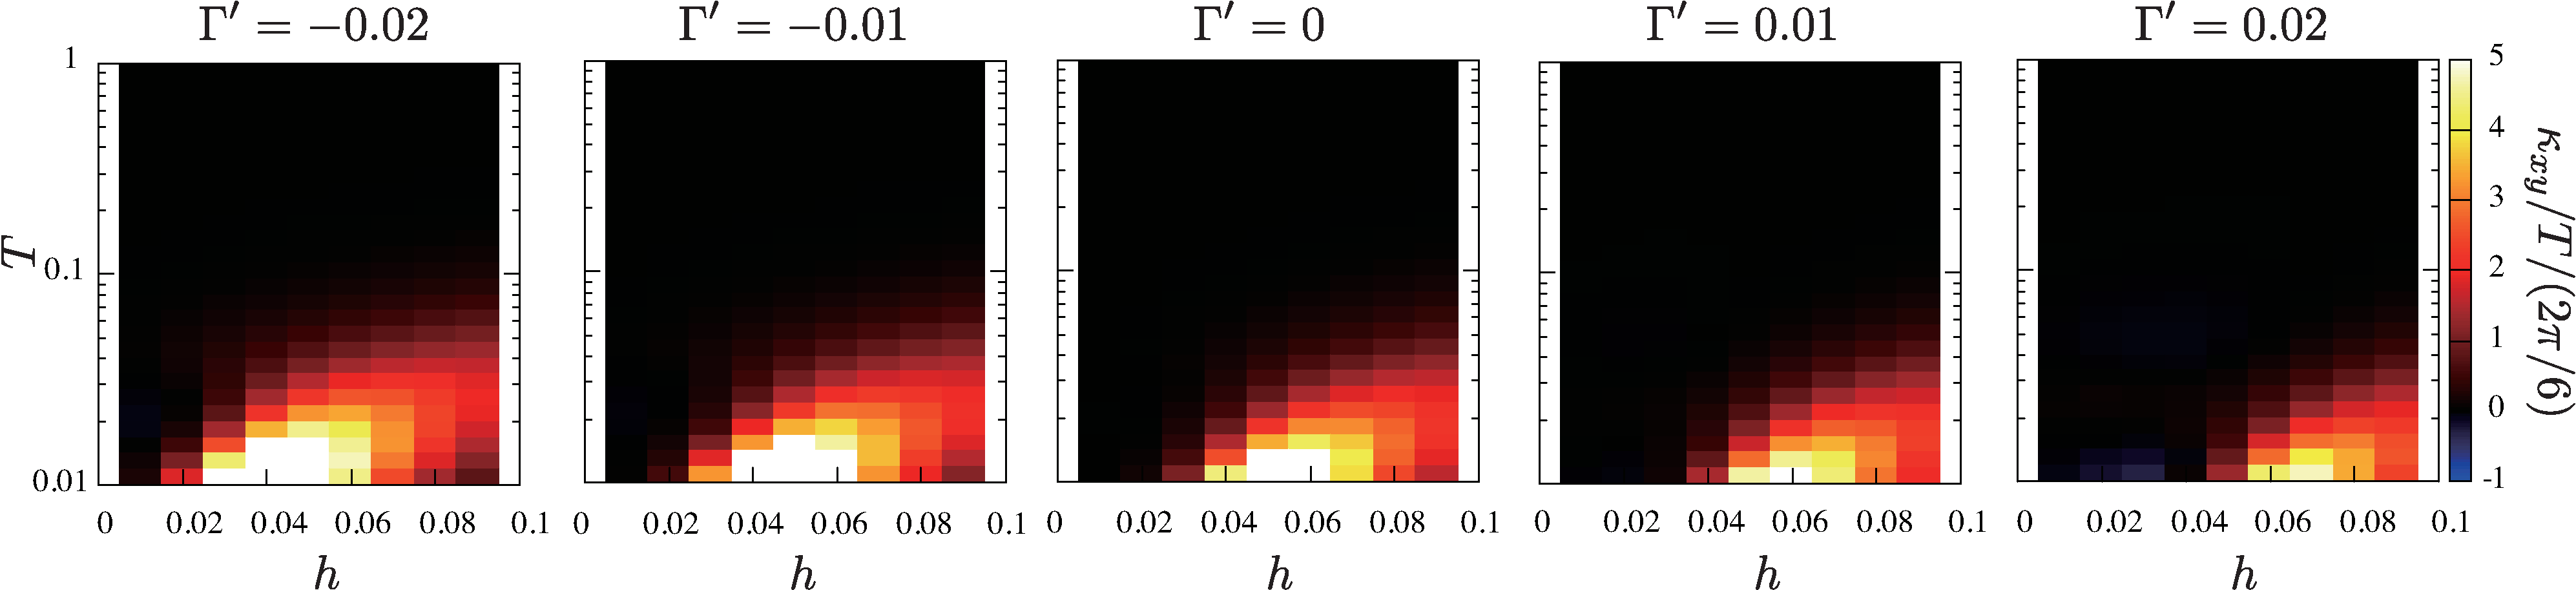
\includegraphics[width=\linewidth]{color_map_Gp_XC4.pdf}
  \end{center}
  \caption{Color maps of $\kappa_{xy}/T$ for ferromagnetic Kitaev model with $\Gamma' = 0, \pm 0.01, \pm 0.02$ with various magnetic fields and temperatures. The lattice is XC4, $L=8$.}
  \label{fig:color_map_Gp_XC4}
\end{figure*}

\section{Benchmark on thermal pure quantum state}
We compare the results of the cTPQ method with
the full diagonalization for the XC4L2 cluster (the total system size is $N_{\rm s}=16$).
In the full exact diagonalization (full ED) method, we diagonalize Hamiltonian whose dimension is
$2^{16}=65536$ using ScaLAPACK. 
After obtaining all the eigenvalues and eigenvectors,
we calculate the temperature dependence of the 
physical quantities.

The definitions of the physical quantities are given as
\begin{align}
C&= \frac{\langle H^2\rangle-\langle H\rangle^2}{T^2}, \\
m&= (m_{x}^2+m_{y}^2+m_z^2)^{1/2}, \\
\kappa&= \frac{d J_{E}}{dT}, \\
J_{E} &= i[H,\vec{P}_{E}] \\ \notag
&=\sum_{[ijk]_{\gamma\gamma^{\prime}}}
\frac{\vec{r}_k-\vec{r}_i}{2}L_{ijk}^{\gamma\gamma^{\prime}}+
\sum_{\langle ij\rangle_{\gamma}}
\frac{\vec{r}_j-\vec{r}_i}{2}M_{ij}^{\gamma}, \\
L_{ijk}^{\gamma\gamma^{\prime}}&=\sum_{\alpha\beta\alpha^{\prime}\beta^{\prime}\gamma{\prime\prime}}
J_{\alpha\beta}^{\gamma}
J_{\alpha^{\prime}\beta^{\prime}}^{\gamma^{\prime}}
\epsilon_{\alpha\gamma^{\prime\prime}\alpha^{\prime}}
S_{i}^{\beta}S_{j}^{\gamma^{\prime\prime}}S_{k}^{\beta^{\prime}}, \\
M_{ij}^{\gamma}&= \sum_{\alpha\beta\gamma^{\prime}\gamma^{\prime\prime}}
J_{\alpha\beta}^{\gamma}h_{\gamma^{\prime}}\epsilon_{\gamma^{\prime}\alpha\gamma^{\prime\prime}}
(S_{i}^{\gamma^{\prime\prime}}S_{j}^{\beta}-S_{i}^{\beta}S_{j}^{\gamma^{\prime\prime}}).
\end{align}

At $|h|=0.04$, the specific heat has three-peak structures.
This three structure may be the finite-size effects 
since it vanishes for larger system sizes. %such as XC6L2.
Even at $|h|=0.08$, the hump in the specific heat 
still exists around $T=0.02$.
As shown in Fig.~\ref{comp_ED}(a),
the cTPQ method reproduces the temperature dependences 
of the specific heat for $|h|=0.04$ and $|h|=0.08$ including
the multiple peak structures.
Fig.~\ref{comp_ED}(b) shows 
the temperature dependence of the magnetization and
the cTPQ method also reproduces the results of the 
full exact diagonalization. 

\begin{figure}[t] 
\begin{center} 
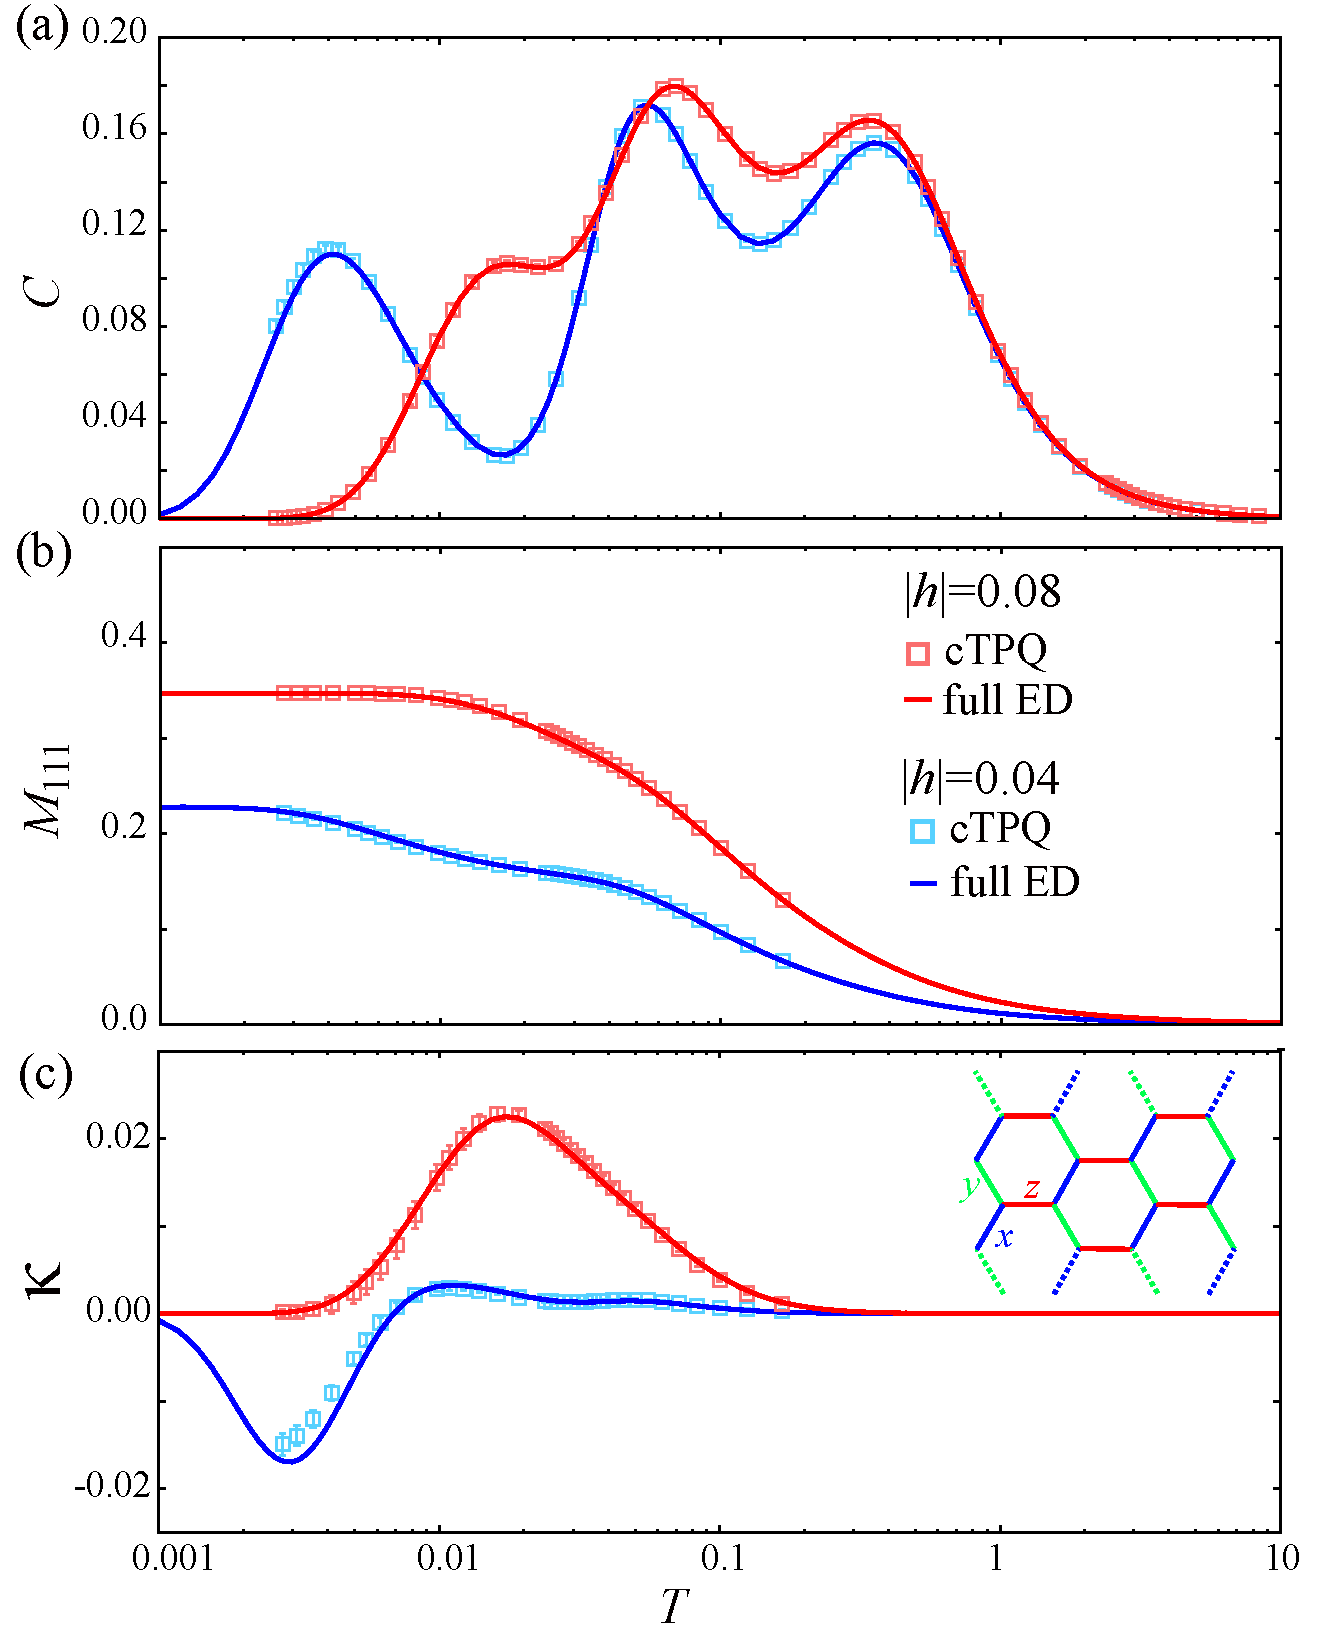
\includegraphics[width=0.9\linewidth]{compED_4_o.pdf}
\vspace{-0.5cm} 
\caption{Temperature dependence of (a) the specific heat, (b) the total magnetization, and
(c) the thermal Hall conductivity $\kappa$.
We take $N_{\rm tot}=P=100,M=50$ ($N_{\rm tot}=P=500,M=250$) 
for $|h|=0.04$ ($|h|=0.08$)
in the bootstrap sampling.}
\label{comp_ED}
\end{center}
\end{figure}


We show the temperature dependence of the thermal 
Hall conductivity $\kappa$ in Fig.~\ref{comp_ED}(c).
The thermal Hall conductivity $\kappa$ at $|h|=0.04$
becomes negative below $T\leq 10^{-2}$. The negative $\kappa$ also may be 
caused by the finite size effects due to short length of the edges.
In fact, $\kappa$ becomes positive for larger system sizes as we show later.
The cTPQ method well reproduces this peculiar temperature 
dependence. At $h=0.08$, the thermal Hall shows 
a single peak structure and it is also well reproduced by the 
cTPQ method.
These consistencies with the results by the full ED demonstrate
the validity of the cTPQ method.
%\tr{{\bf for h=0.08, the agreement is not good. so, I now taking more samples.}}

\section{Comparison between tensor network method and thermal pure quantum state}
Here, we compare the results of the cTPQ method with those of the XTRG
for the XC6L2 cluster ($N_{\rm s}=24$). 
Fig.~\ref{comp_XTRG}(a) shows the temperature dependence of the specific heat. 
We find that both methods reproduce 
the two-peak structure in the specific heat, which is a 
characteristic feature in the Kitaev model. 
Except for the small discrepancy around the low-temperature peak 
at $|h|=0.04$, both independent methods agree well with each other
over the three magnitudes of the temperature scale.
This consistency demonstrates the accuracy of the XTRG method.
%Because the high-temperature peak corresponds to the energy scale of the
%formation of the itinerant Majorana fermions, it does
%not 

In Fig.~\ref{comp_XTRG}(b),
we show the temperature dependence of the magnetization.
In all the temperature regions, 
we find that both methods agree well within the error bars.
Since the magnetization is given by the first derivative of the
free energy, its fluctuation is expected to be small.
This may be the reason why the error bars of the magnetization
are smaller than those of the specific heat 
and the thermal Hall conductivity.

We show the temperature dependence of $\kappa$
in Fig.~\ref{comp_XTRG}(c).
The XTRG method well reproduces the 
temperature dependence of $\kappa$ obtained by the cTPQ method.
Although the small deviations on the peak values of $\kappa$ 
would vanish if we increase bond dimension $D$,
the numerical cost becomes huge. 
To perform the comprehensive calculations of the extended Kitaev models 
in a wide range of the parameters,
we take $D=800$ in the XTRG calculations.
As we demonstrate in Fig.~\ref{comp_XTRG}, 
since $D=800$ already gives sufficiently accurate
results of $\kappa$, it is plausible 
the following XTRG calculations correctly capture the essence of the
finite-temperature properties of the extended Kitaev models. 

\begin{figure}[tbh] 
\begin{center} 
%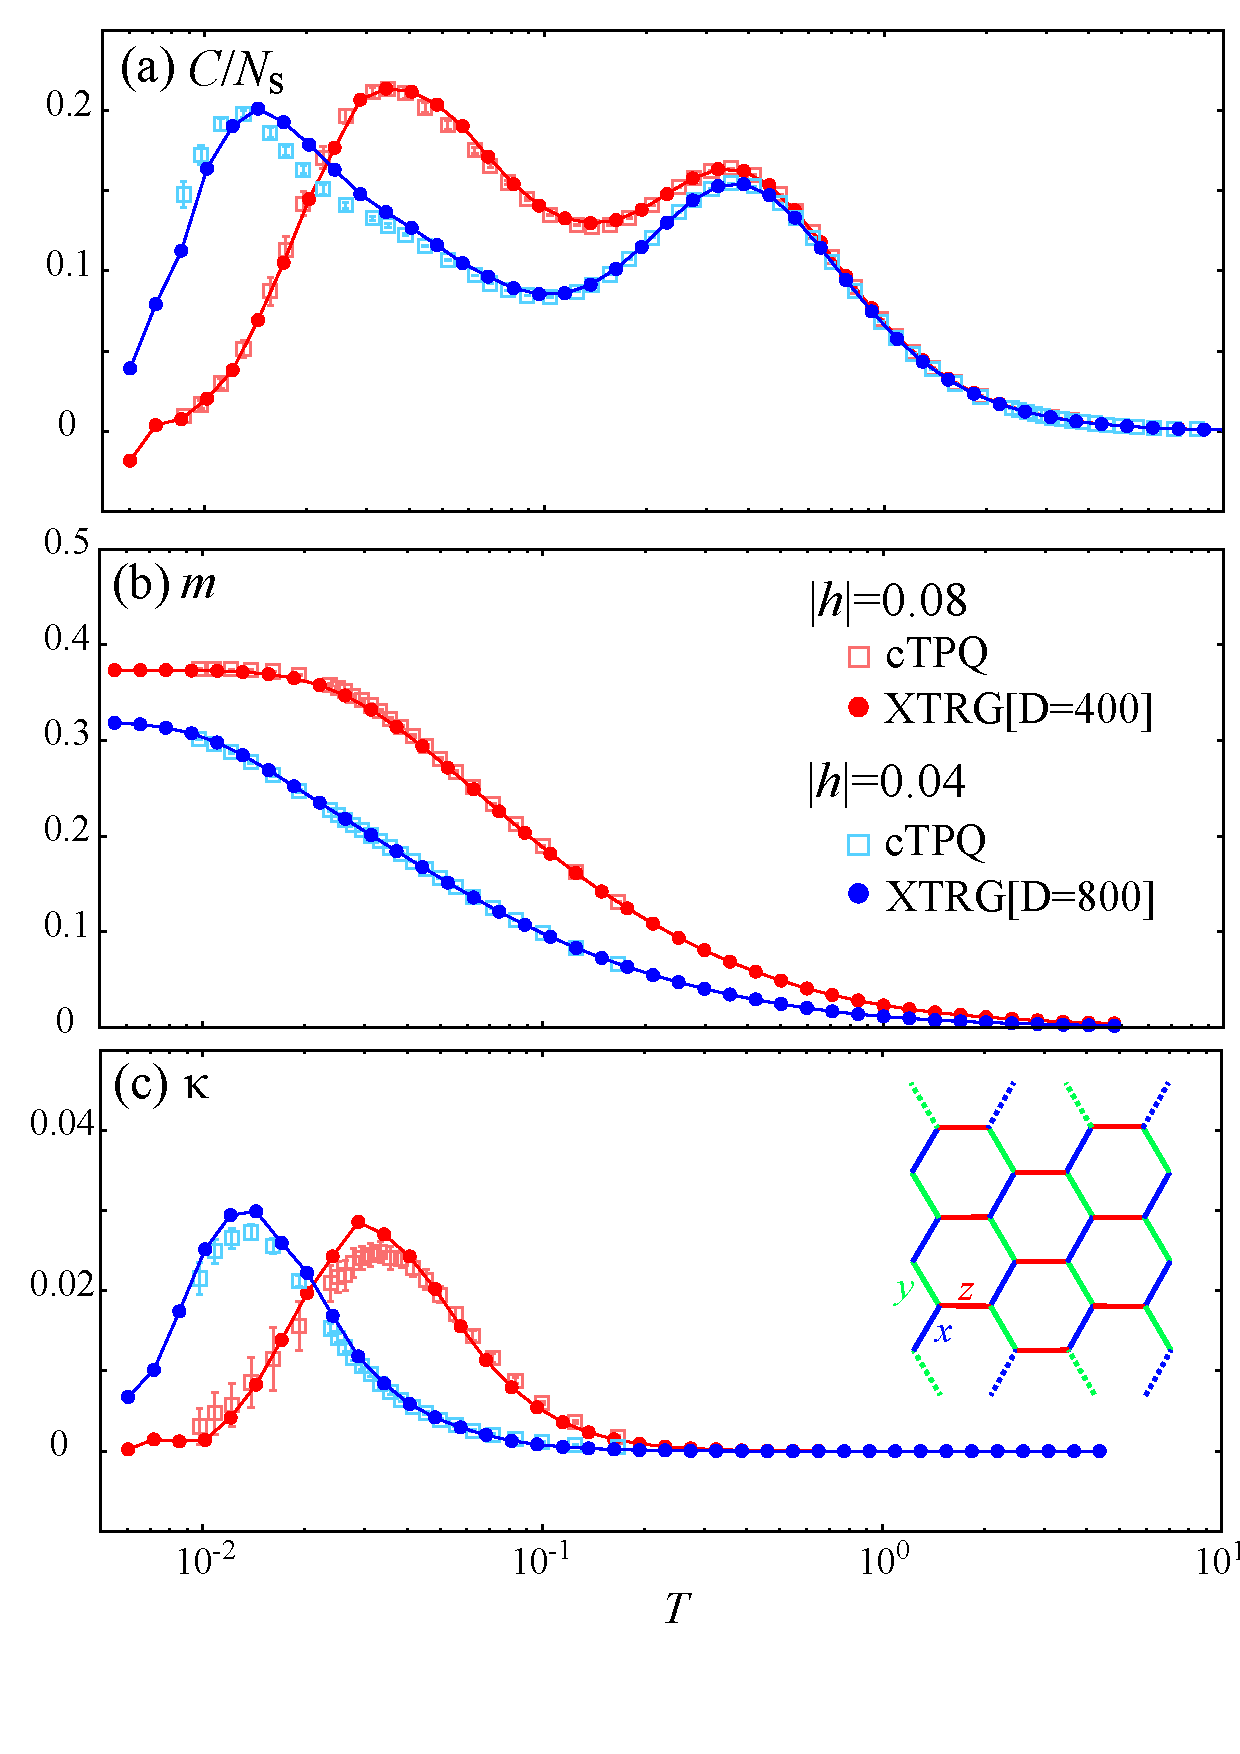
\includegraphics[width=0.9\linewidth]{comp_XTRG_o.pdf}
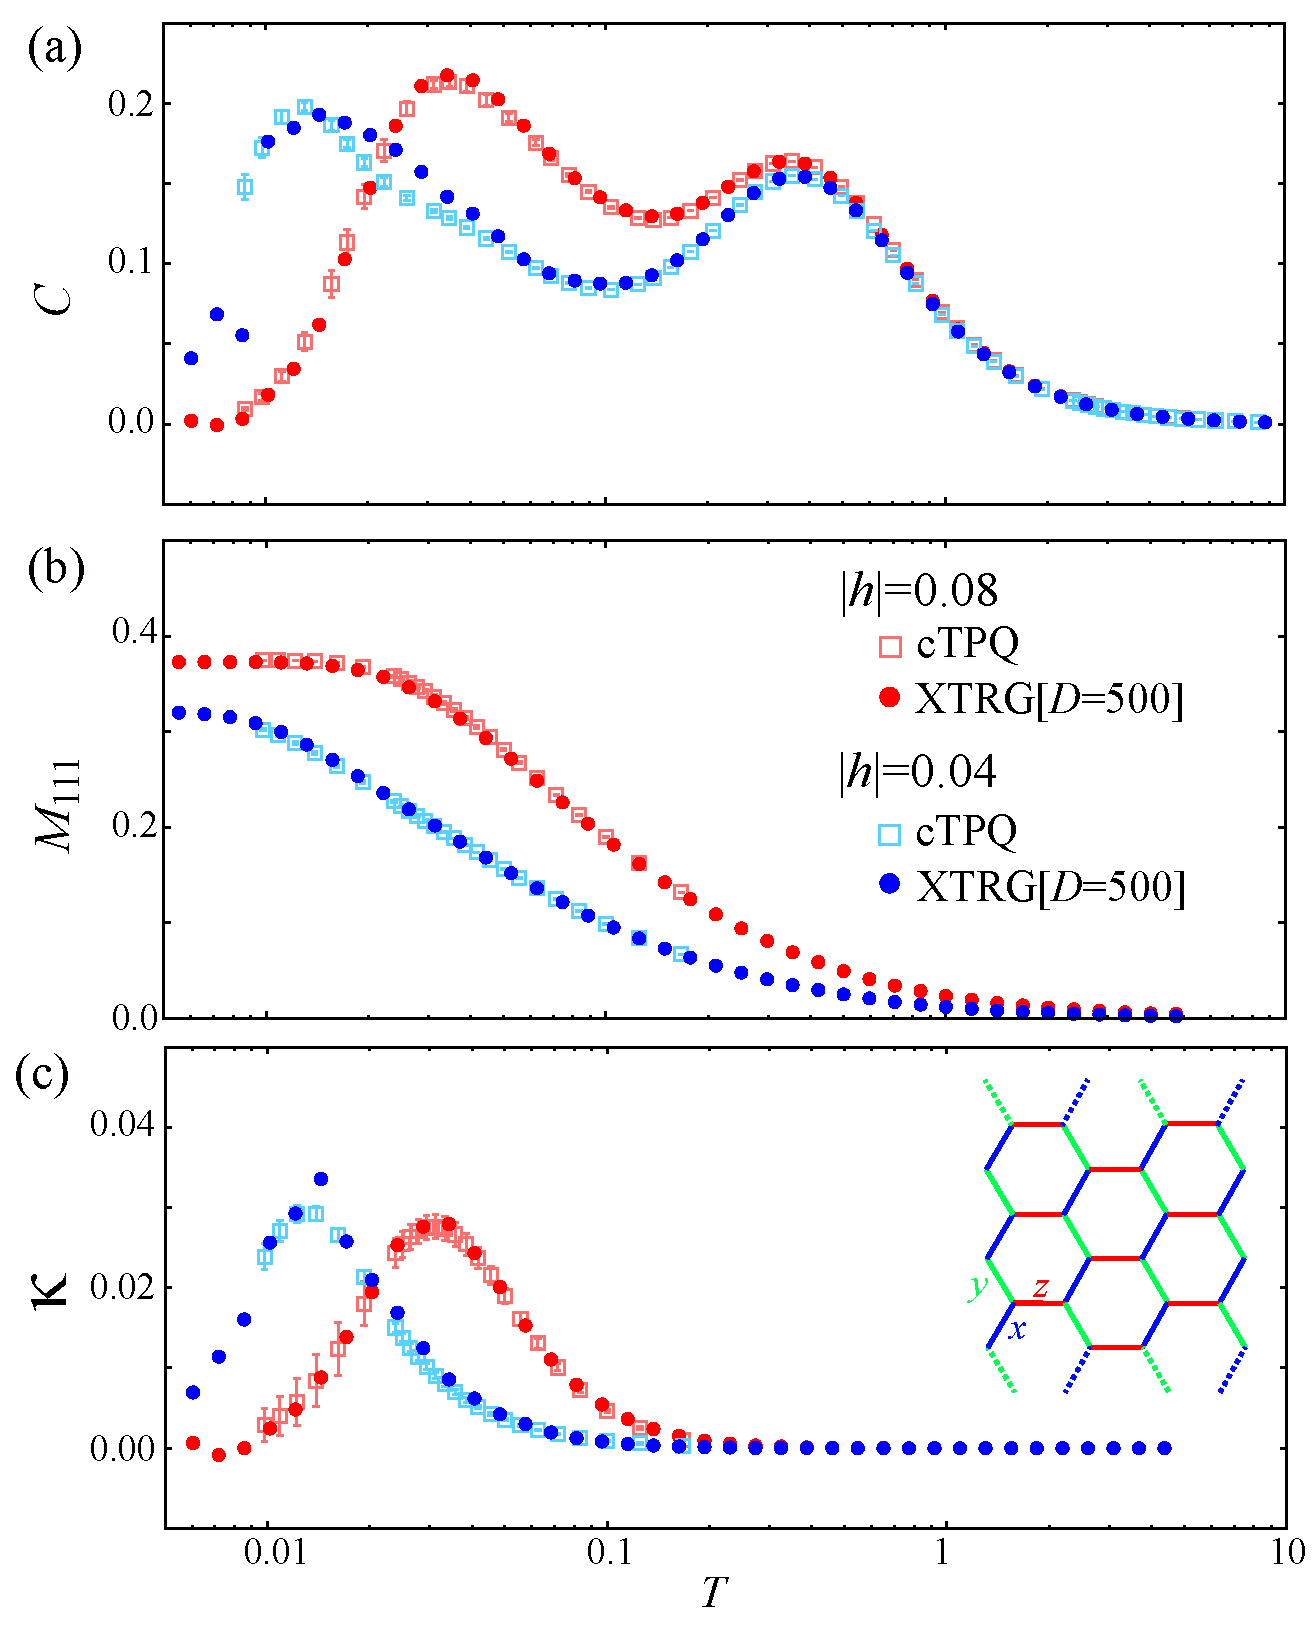
\includegraphics[width=0.9\linewidth]{compXTRG_3_o.pdf}
\vspace{-0.5cm} 
\caption{Temperature dependence of (a) the specific heat, (b) the total magnetization, and
(c) the thermal Hall conductivity $\kappa$. 
We take $N_{\rm tot}=P=100,M=50$ in the bootstrap sampling.}
\label{comp_XTRG}
\end{center}
\end{figure}

\end{document}
